\documentclass[a4paper, 12pt, twoside, openright]{article}
\usepackage[T1]{polski}
\usepackage[utf8]{inputenc}
\newtheorem{theorem}{Twierdzenie}
\usepackage{helvet}
\usepackage{graphicx}
\usepackage{color}
\usepackage{subfig}
\usepackage[table, svgnames, dvipsnames]{xcolor} 
\usepackage{array}
\usepackage{float}
\usepackage{cellspace}
\usepackage[top=1.3in,bottom=1.3in,right=1in,left=1in,headheight=95pt,headsep=-0.5cm]{geometry}
\usepackage{color}
\usepackage{hyperref}
\usepackage{listings}
\usepackage{caption}
\usepackage{cmap}
\newcounter{nalg} 
\DeclareCaptionLabelFormat{algocaption}{Algorytm \thenalg}
\lstnewenvironment{algorithm}[1][] 
{   
	\refstepcounter{nalg}
	\captionsetup{labelformat=algocaption,labelsep=colon} 
	\lstset{ 
		mathescape=true,
		frame=tB,
		numbers=left, 
		numberstyle=\tiny,
		basicstyle=\scriptsize, 
		keywordstyle=\color{black}\bfseries\em,
		keywords={,input, def, output, return, datatype, function, in, if, else, foreach, while, begin, end }
		numbers=left,
		xleftmargin=.04\textwidth,
		#1 
	}
}
{}



\begin{document}

\lstset{language=Python}
% =====  STRONA TYTULOWA  ====

\thispagestyle{empty}
\vspace*{-0.6in}
%% ------------------------ NAGLOWEK STRONY =======================------

\includegraphics[height=37.5mm]{img/logo_agh}\\
\rule{30mm}{0pt}
{\large\textsf{Wydział Fizyki i Informatyki Stosowanej}}\\
\rule{\textwidth}{3pt}\\
\rule[2ex]
{\textwidth}{1pt}\\
\vspace{7ex}
\begin{center}
{\bf\LARGE\textsf{Praca inżynierska}}\\
\vspace{13ex}
% ======================= IMIE I NAZWISKO =======================----
{\bf\Large\textsf{Klaudia Fil}}\\
\vspace{3ex}
{\sf \small kierunek studiów:} {\bf\small\textsf{informatyka stosowana}}\\
\vspace{15ex}
%% ------------------------ TYTUL PRACY =======================-----------
{\bf\huge\textsf{Problem chińskiego listonosza\\ w sieci ulic w Krakowie}}\\
\vspace{14ex}
%% ------------------------ OPIEKUN PRACY =======================---------
{\sf \Large Opiekun:} {\bf\Large\textsf{dr hab. inż. Przemysław Gawroński}}\\
\vspace{22ex}
\textsf{\bf\large\textsf{Kraków, styczeń 2021}}
\end{center}


\newpage

%% =====  Oświadczenie =========
\begin{center}
	{\bf\large\textsf{Oświadczenie studenta}}
\end{center}


{\sf 
	Uprzedzony(-a) o odpowiedzialności karnej na podstawie art. 115 ust. 1 i 2 ustawy z dnia 4 lutego 1994 r. o prawie autorskim i prawach pokrewnych (t.j. Dz. U. z 2018 r. poz. 1191 z późn. zm.): „Kto przywłaszcza sobie autorstwo albo wprowadza w błąd co do autorstwa całości lub części cudzego utworu albo artystycznego wykonania, podlega grzywnie, karze  ograniczenia wolności albo pozbawienia wolności do lat 3. Tej samej karze podlega, kto rozpowszechnia bez podania nazwiska lub pseudonimu twórcy cudzy utwór w wersji oryginalnej albo w postaci opracowania, artystyczne wykonanie albo publicznie zniekształca taki utwór, artystyczne wykonanie, fonogram, wideogram lub nadanie.”, a także uprzedzony(-a) o odpowiedzialności dyscyplinarnej na podstawie art. 307 ust. 1 ustawy z dnia 20 lipca 2018 r. Prawo o szkolnictwie wyższym i nauce (Dz. U. z 2018 r. poz. 1668 z późn. zm.) „Student podlega odpowiedzialności dyscyplinarnej za naruszenie przepisów obowiązujących w uczelni oraz za czyn uchybiający godności studenta.”, oświadczam, że niniejszą pracę dyplomową wykonałem(-am) osobiście i samodzielnie i nie korzystałem(-am) ze źródeł innych niż wymienione w pracy

\bigskip

	Jednocześnie Uczelnia informuje, że zgodnie z art. 15a ww. ustawy o prawie autorskim i prawach pokrewnych Uczelni przysługuje pierwszeństwo w opublikowaniu pracy dyplomowej studenta. Jeżeli Uczelnia nie opublikowała pracy dyplomowej w terminie 6 miesięcy od dnia jej obrony, autor może ją opublikować, chyba że praca jest częścią utworu zbiorowego. Ponadto Uczelnia jako podmiot, o którym mowa w art. 7 ust. 1 pkt 1 ustawy z dnia 20 lipca 2018 r. — Prawo o szkolnictwie wyższym i nauce (Dz. U. z 2018 r. poz. 1668 z późn. zm.), może korzystać bez wynagrodzenia i bez konieczności uzyskania zgody autora z utworu stworzonego przez studenta w wyniku wykonywania obowiązków związanych z odbywaniem studiów, udostępniać utwór ministrowi właściwemu do spraw szkolnictwa wyższego i nauki oraz korzystać z utworów znajdujących się w prowadzonych przez niego bazach danych, w celu sprawdzania z wykorzystaniem systemu antyplagiatowego. Minister właściwy do spraw szkolnictwa wyższego i nauki może korzystać z prac dyplomowych znajdujących się w prowadzonych przez niego bazach danych w zakresie niezbędnym do zapewnienia prawidłowego utrzymania i rozwoju tych baz oraz współpracujących z nimi systemów informatycznych.}

\vspace{15ex}

\begin{center}

~~~~~~~~~~~~~~~~~~~~~~~~~~~~~~~~~~~~~~~~~~~~~~~~~~~~~~~~~~~~~~~~~ 
................................................................. \\
~~~~~~~~~~~~~~~~~~~~~~~~~~~~~~~~~~~~~~~~~~~~~~~~~~~~~~~~~~~~~~~  {\sf (czytelny podpis)} \\

\end{center}

%% =====  TYL STRONY TYTULOWEJ   ====


%% ============ OCENA OPIEKUNA =============
\newpage
\linespread{1.3}
\selectfont

\hspace*{\fill}\large{Ocena merytoryczna opiekuna}

\vspace{85mm}

%% ============ OCENA RECENZENTA =============
\newpage
\linespread{1.3}
\selectfont

\hspace*{\fill}\large{Ocena merytoryczna recenzenta}

\vspace{85mm}


%% ====== SPIS TRESCI ==========
\newpage
\tableofcontents


%=======================- 1 =======================
\newpage
\section{Wstęp}
\subsection{Wprowadzenie}
	\indent\par
	Szeroko pojęty problem związany z wyznaczaniem trasy (ang. \textit{General Routing Problem}) zdefiniowano jako szukanie drogi o minimalnym koszcie, która dodatkowo musi spełniać uwzględnione w planowaniu wymagania$^{\cite{varianntsCPP}}$.
	Skupiając się na praktycznym aspekcie GRP należy wziąć pod uwagę jeden z bardziej znanych przypadków rozważań - problem chińskiego listonosza (ang. \textit{Chinese Postman Problem})$^{\cite{arcRoutingProblemsPart1}}$. 


	W życiu codziennym wiele zawodów związanych jest z wyznaczaniem trasy na tle procesów logistycznych, wśród nich różnego rodzaju dostawcy, kurierzy czy właśnie listonosze. Ich szlakiem docelowym jest droga zawierająca w sobie każdą ulicę danego obszaru przynajmniej raz. Optymalnym rozwiązaniem CPP byłoby uniknięcie ponownych przejść jedną ścieżką, jednak w sytuacjach rzeczywistych jest to często niemożliwe.

\subsection{Cel pracy}
	\indent\par
	Celem pracy dyplomowej jest zaimplementowanie dwóch algorytmów, rozwiązujących kwestię znajdowania pełnej ścieżki z cyklem zamkniętym na grafie spójnym, przy optymalizacji kosztów przemieszczania się, co sprowadza się do CPP. 
	Rozpatrzono w niej przypadki rzeczywiste, gdzie w powstałych z mapy Krakowa grafach mieszanych (ang. \textit{Mixed Graph}) (nazywanych również ogólnie jako grafy skierowane (ang. \textit{Directed Graph})) oraz nieskierowanych (ang. \textit{Undirected Graph}), znajdowana jest najlepsza droga dla listonosza$^{\cite{mixedGraph}}$.


	Jeden z algorytmów przedstawiony w pracy dedykowany jest MG. Swoje zastosowanie ma, kiedy przebieg trasy listonosza uwarunkowany jest czynnikami zewnętrznymi tj. drogami jedno- lub dwukierunkowymi. 
	W przypadku pieszego ruchu, w którym sposób przejścia jest  dowolny, problem dotyczy UG. Zaimplementowano dla niego drugi z schematów umożliwiający wyznaczenie najbardziej efektywnej trasy. Graf rzeczywisty tworzony jest z małych fragmentów miasta, dlatego założono, że poruszać się będzie po nim tylko jeden listonosz. 


	Dla sprawdzenia poprawności oraz wyznaczenia złożoności algorytmów wygenerowano losowe sieci, które pozwoliły na szersze ich przetestowanie. 
	Stworzono również program do wizualizacji grafów, oraz kolejnych etapów ścieżek, umożliwiający graficzne prześledzenie działania schematów.




\subsection{Problemu chińskiego listonosza}
	\indent\par
	Problem chińskiego listonosza jest jedynym z podstawowych zagadnień związanych z wyznaczaniem trasy. Swoją nazwę zawdzięcza chińskiemu matematykowi, który jako pierwszy go sformułował. Analizował drogę dostawcy w jednym z chińskich miast, który miał dostarczyć wszystkie przesyłki, odwiedzając każdą ulice, nie nadkładając niepotrzebnie drogi i powrócić do bazy$^{{\cite{CPP}}}$. 
	
	Patrząc przez pryzmat przypadku rzeczywistego, gdzie rozważany jest listonosz, czy dostawca ulotek, CPP sprowadza się do procesu wyboru najlepszej ścieżki w sieci dróg, gdzie  każda ulica musi zostać odwiedzona przynajmniej raz, czyli odnalezienia na grafie cyklu Eulera$^{\cite{MatchingEulertourAsCPP}}$. 

\subsection{Cykl Eulera} \label{SciezkaEulera}

\indent\par
	Cykl Eulera (ang. \textit{Eulerian Cycle}) jest to ścieżka poprowadzona na dowolnym grafie, która przechodzi przez każdą z krawędzi dokładnie raz. Nazywamy ją cyklem, ponieważ zaczyna się i kończy w tym samym wierzchołku. 
	
	Nazwa takiego przejścia przez graf nadana została na cześć matematyka Leonharda Eulera, który w swojej pracy \textit{Solutio problematis ad geometriam situs pertinentis}$^{\cite{euler}}$ poruszył zagadnienie mostów królewieckich. Odpowiadał na pytanie, czy istnieje ścieżka prowadząca przez wszystkie mosty, biorąc pod uwagę, że przez każdy z nich można iść tylko raz. 
	
	\begin{figure}[H]
		\centering
		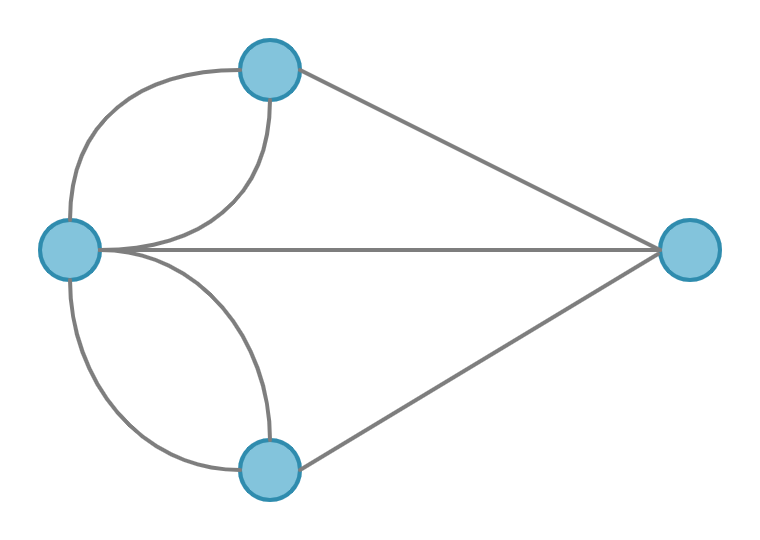
\includegraphics[width=0.5\textwidth]{img/wstep/w1}
		\caption[]{Graf przestawiający problem mostów w Królewcu\footnotemark.}
		\label{krolewiec}
	\end{figure}
	\footnotetext{Graf wygenerowany przy pomocy strony internetowej \href{https://creately.com/}{https://creately.com/}}
	
	Mapa, którą rozważał, sprowadzała się do grafu z rysunku \ref{krolewiec}, gdzie krawędzie odpowiadają siedmiu mostom. Wykazał, że znalezienie EC jest możliwe tylko dla grafów spełniających określone warunki, nazwanych na jego cześć grafami Eulera. Była to jedna z pierwszych prac związanych z teorią grafów.
	
	\subsubsection{Graf Eulera} \label{grafEulera}
	\begin{theorem}[Euler, 1736]
		\label{twEuleraUG}
		Graf spójny jest eulerowski wtedy i tylko wtedy, gdy
		stopień każdego wierzchołka jest liczbą parzystą.	
	\end{theorem}

	 \begin{theorem}
	 	\label{twEuleraDG}
	 	Graf skierowany spójny zawiera cykl Eulera wtedy i tylko wtedy, gdy
	 	dla każdego wierzchołka v zachodzi $d ^{+} (v) = d ^{-} (v) $, gdzie \indent\par$d ^{+} (v)$ - ilość krawędzi wchodzących do wierzchołka v, \indent\par$d ^{-} (v)$ - ilość krawędzi wychodzących z wierzchołka v.
	 \end{theorem}
 
	 Aby możliwe było znalezienie poprawnej ścieżki dzięki opisanym w tej pracy algorytmom, grafy w nich wykorzystywane muszą spełniać twierdzenia \ref{twEuleraUG} i \ref{twEuleraDG}. 
	 

\subsection{Sieci złożone} \label{SieciZlozone}
\subsubsection{Sieć Barabási–Albert}\label{BarabasiAlbert}
\indent\par

 	Pod koniec XX w. na Uniwersytecie Notre Dame w Indianie Reka Albert i Albert-Laszlo Barabasi podczas badania struktury sieci WWW przypadkiem odkryli ciekawą zależność, a mianowicie potęgowe rozkłady prawdopodobieństwa opisujące połączenia pomiędzy stronami internetowymi.
 
	 Rozkład ten wyglądał następująco:
 	\begin{equation}
 		\label{eqn:rozkladP}
 		P(k) \sim k ^{-\alpha}
 	\end{equation}
 
 	co oznaczało, że sieć WWW ma własności fraktalne.

 	Zauważono, że większość układów rzeczywistych również charakteryzuje się rozkładem podobnym do równania \ref{eqn:rozkladP}. Szerszą analizę i reguły tworzenia sieci tego typu panowie Albert i Barabasi przedstawili w swojej pracy zatytułowanej \textit{Emergence of scaling in random networks}$^{\cite{barabasiAlbert}}$. Ustalili, że rozkład \ref{eqn:rozkladP} wynika ze wzrostu sieci i reguły związanej z preferencyjnym dołączaniem węzłów.
 	
 
	Formułowanie ewoluującej sieci polega na stopniowym jej rozroście w każdym momencie czasowym. Proces rozpoczęty w chwili zerowej składa się z grafu zawierającego $m_0$ połączonych wierzchołków. Podczas kolejnych kroków czasowych nowo dodawany węzeł łączony jest z $m$ innymi, istniejącymi już wierzchołkami.	Szansa, że świeżo utworzony wierzchołek połączony zostanie krawędzią do starego węzła jest proporcjonalne do stopnia węzła $k_i$:
	
	\begin{equation}
		\Pi (k_i) = { k_i \over {\sum_{i=1}^{t} k_i} }
	\end{equation}
	co przedstawione jest na rysunku \ref{BarabasiImg1}.
	

	\captionsetup{justification=centering}
	\begin{figure}[!p]
		\centering
		\subfloat[$m_0=1$, $t=3$]{\label{b_a}
			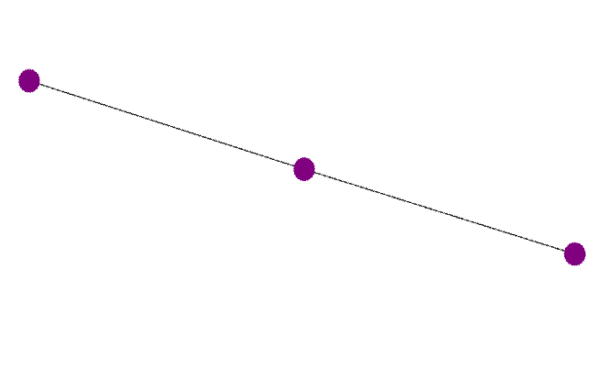
\includegraphics[width=0.4\textwidth]{img/wstep/bara_1a.png}}
		\quad
		\subfloat[$m_0=1$, $t=6$]{\label{b_b}
			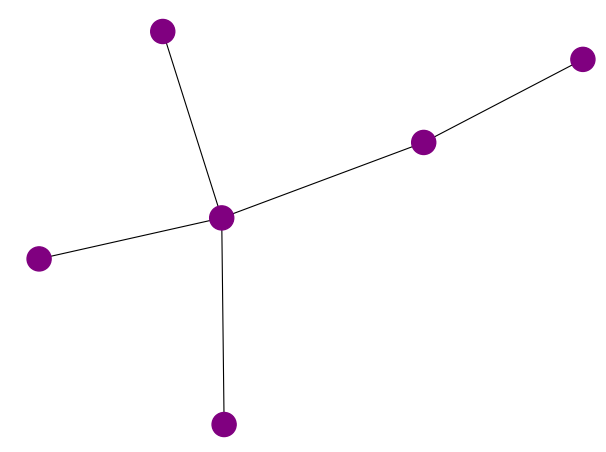
\includegraphics[width=0.4\textwidth]{img/wstep/bara_1b.png}}
		\quad
		\subfloat[$m_0=1$, $t=10$]{\label{b_c}
			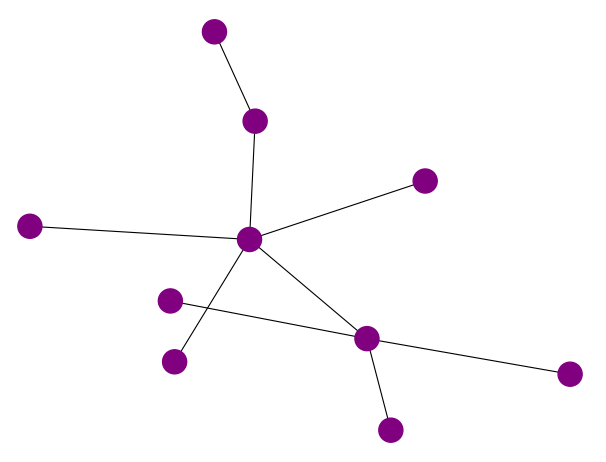
\includegraphics[width=0.4\textwidth]{img/wstep/bara_1c.png}}
		\quad
		\subfloat[$m_0=1$, $t=15$]{\label{b_d}
			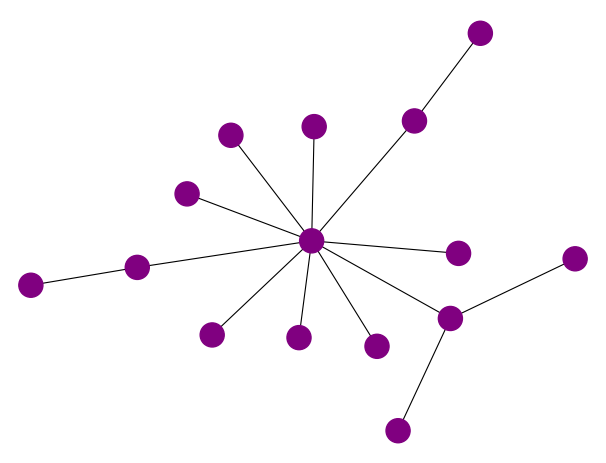
\includegraphics[width=0.4\textwidth]{img/wstep/bara_1d.png}}
		\quad
		\subfloat[$m_0=1$, $t=30$]{\label{b_e}
			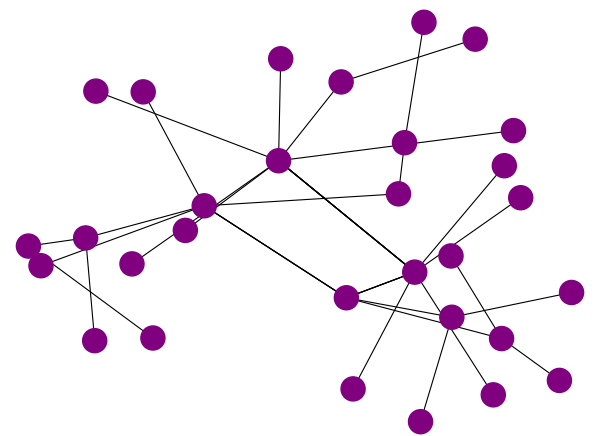
\includegraphics[width=0.4\textwidth]{img/wstep/bara_1e.png}}
		\quad
		\subfloat[$m_0=1$, $t=50$]{\label{b_f}
			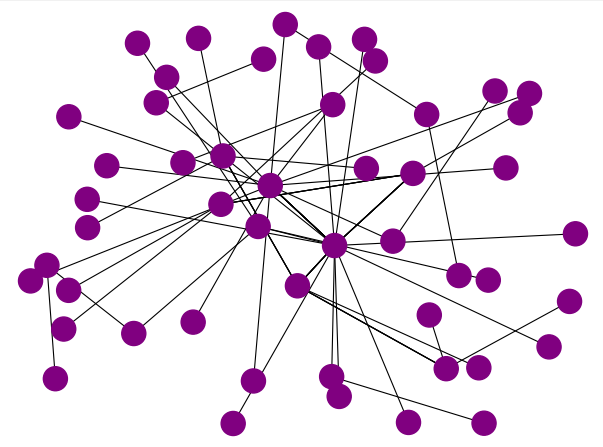
\includegraphics[width=0.4\textwidth]{img/wstep/bara_1f.png}}		
		
		\caption[]{Graf losowy stworzony zgodnie z modelem Barabási–Albert o początkowych wierzchołkach $m_0$ w kolejnych krokach czasowych $t$.}
		\label{BarabasiImg1}
	\end{figure}
 	
 	
 	Algorytm, z którego skorzystano w pracy, tworzący grafy w wyżej opisanym modelu to \textit{barabasi\char`_albert\char`_graph}, zaczerpnięto go z biblioteki \textit{Networkx} szerzej opisanej w rozdziale \ref{narzedzia}.
	
	
\subsubsection{Sieć Wattsa–Strogatza} \label{WSWS}
\indent\par
	W 1967 r. psycholog Stanley Milgram przeprowadził eksperyment \textit{Small-world project}$^{\cite{smallWorldProj}}$, który opisuje połączenia w dużej społeczności. Zaobserwował on, że większość osób potrzebuje niewielkiej liczby przyjaciół, którzy mogą przedstawić ich swoim znajomym, umożliwiając poznanie całej badanej grupy. Wyniki eksperymentu nazwano \textit{hipotezą o małym świecie}, co oznacza, że każdego człowieka łączy stosunkowo niewielka liczba pośredników w danym społeczeństwie.
	
	Charakterystyka modelu grafu, która wyjaśnia zjawisko zaobserwowane przez Milgrama, została zaproponowana w 1998 r. przez Duncana Wattsa i Stephena Strogatza w pracy \textit{Collective dynamics of ‘small-world’ networks}$^{\cite{wattsS_bib}}$. 
	
	Struktura grafy powstaje z sieci regularnej, w której wprowadzona zostaje randomizacja wierzchołków. Ponadto, aby została ona zakwalifikowany do kategorii \textit{small-world}, jej parametry: współczynnik klastrowania ${C_g}^{\Delta}$ zadany wzorem
	\begin{equation}
		\label{klastracja}
		{C_g}^{\Delta}  = {{3t} \over {k}},
	\end{equation}
	\par gdzie:\indent\par 
	$t$ - liczba węzłów tworzących \textit{trójkąty}, czyli trzech wierzchołków połączonych każdy z każdym,\indent\par
	$k$ - liczba ścieżek o długości 2,\\
	 oraz średnia odległość pomiędzy dowolną parą wierzchołków $L_g$ muszą spełniać wymogi twierdzenia \ref{ctwWS}$^{\cite{ws_wzor}}$. 
	\newpage
	\begin{theorem}
		\label{ctwWS}
		O sieci $G$ mówi się, że jest siecią typu \textit{mały świat}, jeżeli $L_g \ge L_{rand}$ oraz ${C_g}^{\Delta} \gg {C_{rand}}^{\Delta}$, \\gdzie\indent\par
		$L_g$ - najkrótsza ścieżka grafu G,\indent\par
		$L_{rand}$ - najkrótsza ścieżka pomiędzy dwoma węzłami losowego grafu, stworzonego z takiej samej ilości wierzchołków i krawędzi jak graf G, zachowując przy tym prawdopodobieństwo przypisania krawędzi do pary węzłów,\indent\par
		${C_g}^{\Delta}$ - współczynnik klastrowania grafu G, wyznaczony ze wzoru \ref{klastracja},\indent\par
		${C_{rand}}^{\Delta}$ - współczynnik klastrowania grafu losowego, stworzonego z takiej samej ilości wierzchołków i krawędzi jak graf G, zachowując przy tym prawdopodobieństwo przypisania krawędzi do pary węzłów.
	\end{theorem}
	Wykorzystując twierdzenie \ref{ctwWS} do wyprowadzenia zależności:
	\begin{equation}
	 	\label{gamma}
		{\gamma_g}^{\Delta} = {{C_g^{\Delta}} \over {C_{rand}^{\Delta}}},
	\end{equation}
 	\begin{equation}
	 	\label{lambda}
	 	{\lambda_g}  = {{L_g} \over {L_{rand}}},
 	\end{equation}
	 sformułowano końcowy postulat:
	\begin{theorem}
		\label{twWS}
		O sieci $G$ mówi się, że jest siecią \textit{małego świata}, jeżeli ${S}^{\Delta} > 1$, \\gdzie \indent\par${S}^{\Delta} = {{{\gamma_g}^{\Delta}} \over {\lambda_g}}$.
	\end{theorem}

	Współczynnik klastrowania określa stopnień wykorzystania wszystkich możliwych połączeń międzywęzłowych. $C$ w praktyce pozwala na ocenienie stopnia oddalenia pomiędzy wierzchołkami$^{\cite{wlasnSieciZloz}}$.
	
	 Algorytm generujący grafy o modelu Wattsa–Strogatza wykorzystany w pracy to \textit{watts\_strogatz\_graph}, który podobnie jak model \ref{BarabasiAlbert} pochodzi z biblioteki \textit{Networkx}.

\captionsetup{justification=centering}
\begin{figure}[!p]
	\centering
	\subfloat[$n=12, k=2, p=0$]{\label{ws_a}
		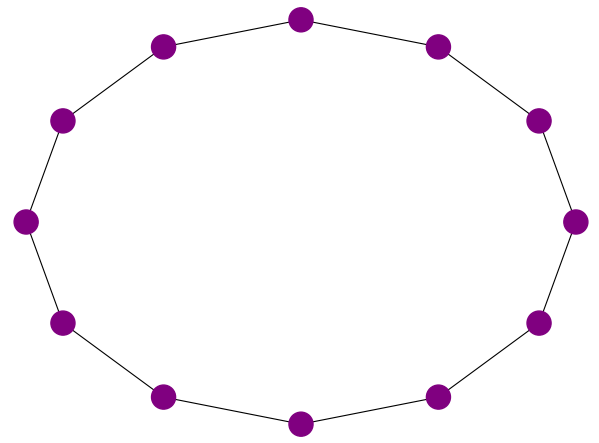
\includegraphics[width=0.35\textwidth]{img/wstep/ws_1a.png}}
	\quad
	\subfloat[$n=12, k=4, p=0$]{\label{ws_b}
		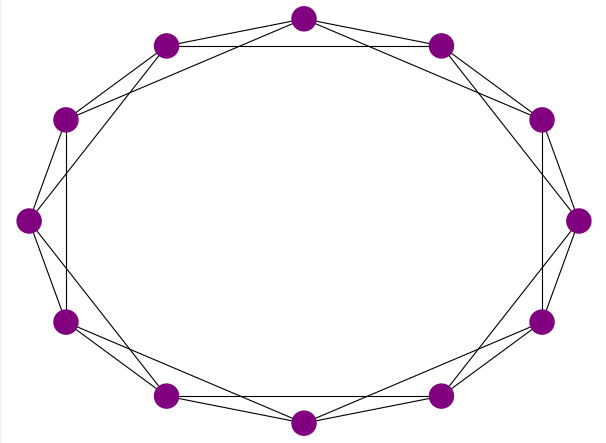
\includegraphics[width=0.35\textwidth]{img/wstep/ws_1b.png}}
	\quad
	\subfloat[$n=12, k=2, p=0.3$]{\label{ws_c}
		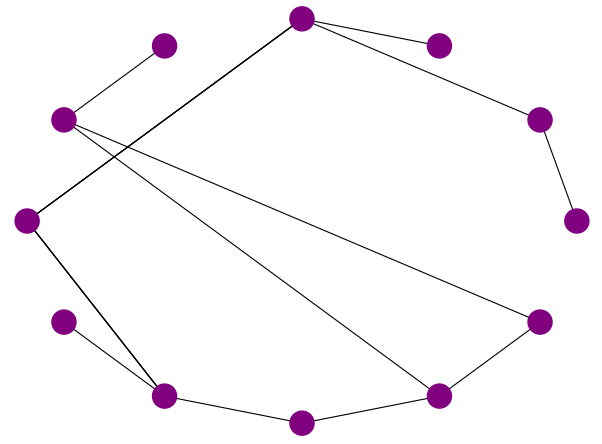
\includegraphics[width=0.35\textwidth]{img/wstep/ws_1c.png}}
	\quad
	\subfloat[$n=12, k=4, p=0.3$]{\label{ws_d}
		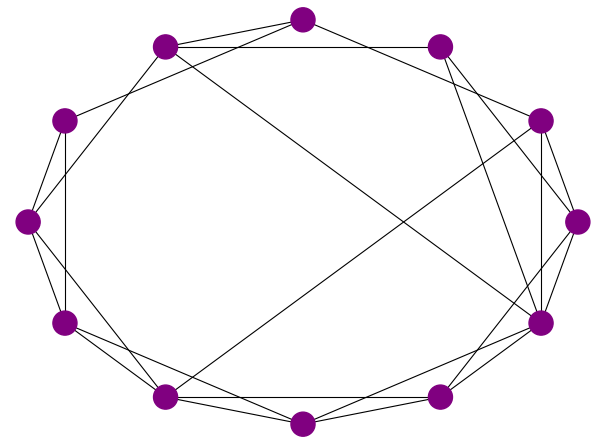
\includegraphics[width=0.35\textwidth]{img/wstep/ws_1d.png}}
	\quad
	\subfloat[$n=12, k=2, p=0.6$]{\label{ws_e}
		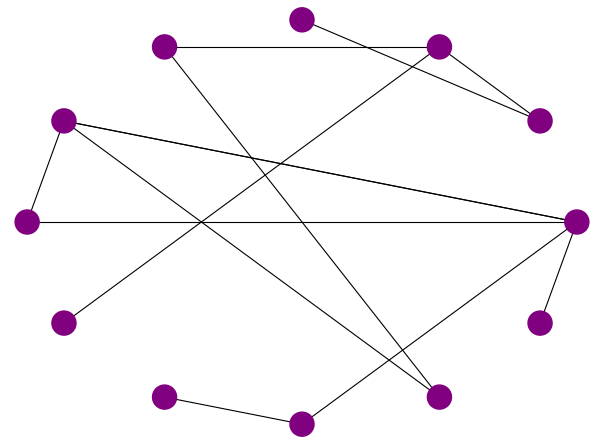
\includegraphics[width=0.35\textwidth]{img/wstep/ws_1e.png}}
	\quad
	\subfloat[$n=12, k=4, p=0.6$]{\label{ws_f}
		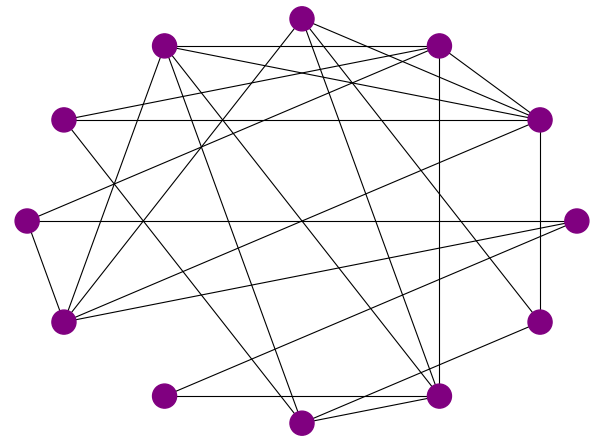
\includegraphics[width=0.35\textwidth]{img/wstep/ws_1f.png}}		
	\quad
	\subfloat[$n=12, k=2, p=1$]{\label{ws_g}
		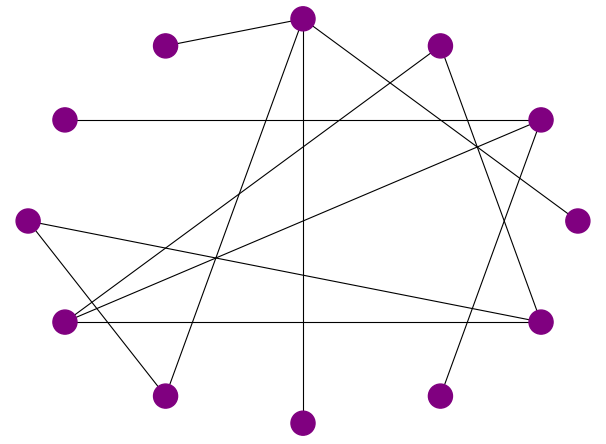
\includegraphics[width=0.35\textwidth]{img/wstep/ws_1g.png}}
	\quad
	\subfloat[$n=12, k=4, p=1$]{\label{ws_h}
		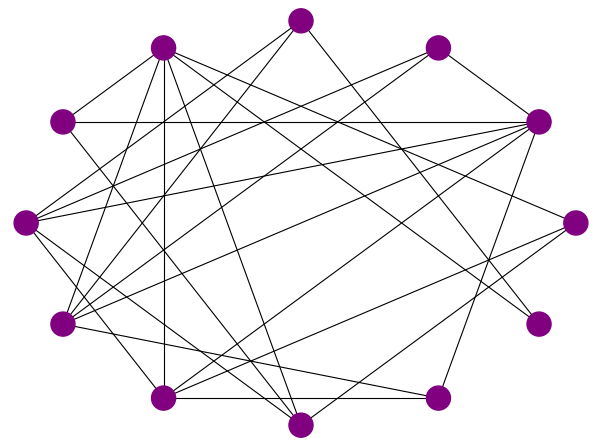
\includegraphics[width=0.35\textwidth]{img/wstep/ws_1h.png}}	
		
	\caption[]{Sieć stworzona zgodnie z modelem Wattsa–Strogatza, gdzie $n$ - liczba wierzchołków, $k$ - ilość najbliższych sąsiadów do połączenia w topologii pierścienia, $p$ - prawdopodobieństwo zmiany połączenia.}
	\label{WattsImg1}
\end{figure}

	Przy tworzeniu losowych grafów zgodnie z modelem Wattsa-Strogatza posłużono się wartościami $n,k,p$, które kolejno oznaczają ilość wierzchołków, ilość połączeń pomiędzy najbliższymi sąsiadami, prawdopodobieństwo zmiany jednego z węzłów krawędzi.
	
	Na rysunku \ref{WattsImg1} przedstawiono wygląd randomizacji wierzchołków w modelu sieci 12-to węzłowej dla dwóch przypadków ilości połączeń: dwóch sąsiadów na \ref{ws_a}, \ref{ws_c}, \ref{ws_e}, \ref{ws_g} oraz czterech na \ref{ws_b}, \ref{ws_d}, \ref{ws_f}, \ref{ws_h}, gdzie każdy kolejny rysunek prezentuje wygląd po losowym przydzieleniu nowych krawędzi dla prawdopodobieństw $p = 0, 0.3, 0.6, 1$, gdzie $p \in [0, 1]$. Wraz z wzrostem $p$ zauważalne jest odejście od początkowej regularności układu przy zerowej wartości. Dla górnego przedziału $p$ sieć praktycznie wcale nie przypomina modelu \textit{small-world}, czego można się spodziewać po odstępstwie od założeń zgodnych z twierdzeniami \ref{ctwWS} i \ref{twWS}.
	

% ======================= 2 =======================
\newpage
\section{Narzędzia} \label{narzedzia}

\indent\par
	Aplikacja w całości została zaimplementowana w Pythonie$^{\cite{python}}$, ze względu na jego prostotę i czytelność, które ułatwiały znacznie pracę. Inną kwestią przemawiającą za tym językiem jest dobrze udokumentowana, ciągle rozwijająca się biblioteka związana z teorią grafów. Kilka algorytmów pochodzących z niej zostało wykorzystane przy pisaniu projektu, m. in. do wyliczania najkrótszych ścieżek przy tworzeniu losowych grafów.

	Biblioteki użyte w pracy:
	\begin{itemize}
		\item \textit{Networkx}$^{\cite{networkx}}$ - biblioteka w języku Python używana przy badaniu i tworzeniu dużych grafów i sieci. Wykorzystana została w algorytmie konwertującym graf do takiego, który posiada ścieżkę Eulera opisaną w \ref{SciezkaEulera} i podczas tworzenia przypadkowego grafu skierowanego oraz sieci złożonych z podpunktu \ref{SieciZlozone}.
		\item \textit{Matplotlib}$^{\cite{matplotlib}}$ - jedna z najbogatszych bibliotek do tworzenia wykresów w języku Python. W pracy gównie posłużono się zawartym w niej API \textit{pylab} wykorzystującym prosty interface analogiczny do środowiska MATLAB$^{\cite{matlab}}$.
	\end{itemize}

	Inną istotną rzeczą użytą w projekcie to mapa świata OpenStreetMap (OSM)$^{\cite{openstreetmap}}$, która zbudowana jest z danych gromadzonych przez szeroką społeczność. Dowolna osoba może przyczynić się do jej rozwoju poprzez dostarczenie informacji geograficznych zbieranych przez urządzenia z odbiornikami GPS lub zdjęcia satelitarne. Dane w niej są udostępnione za darmo do ogólnego użytku.




%======================= 3 =======================
\newpage
\section{Algorytmy i implementacja}

\subsection{Modyfikacja do grafu Eulera} \label{modyfikacja}
\indent\par
	Algorytmy Fleury’ego i Hierholzera mające wyznaczyć ścieżki zakładają, że obiekty, które przeszukują, są grafami Eulera, co opisano szerzej w rozdziale \ref{SciezkaEulera}. Ponieważ dane testowe każdego rodzaju (losowy DG, sieci o modelu Barabásiego–Alberta oraz Wattsa–Strogatza) tworzone są randomowo, przez funkcje biblioteczne \textit{Networkx}, wymagana jest ich modyfikacja, gdyby nie było w nich cyklu Eulera. Na potrzeby tych warunków przeprowadzono implementacje dwóch algorytmów. 
	
\subsubsection{Modyfikacja grafu nieskierowanego} \label{mgnieskier}
	\indent\par	
	W przypadku wygenerowania UG sprawdzane jest pierwsze, czy modyfikacje są wymagane, realizowane jest to przy pomocy funkcji \textit{is\_eulerian} z biblioteki grafowej opisanej w rozdziale \ref{narzedzia}. Kiedy zwracana jest informacja o niezgodności z twierdzeniem \ref{twEuleraUG} wywoływana jest funkcja odpowiedzialna za dodanie duplikatów krawędzi, które zapewnią poprawny stopnień każdego z wierzchołków. 
	
	Początkowo uzupełniana jest lista z nieparzystymi wierzchołkami (linie 4-6 alg. \ref{makeeulerianUG}). Ich nieparzysta ilość uniemożliwia stworzenie połączeń, zwracana jest wartość \textit{None}, która wywołuje mechanizm odpowiedzialny za ponowne wylosowanie wartości, aż modyfikacja będzie możliwa.
	
\begin{algorithm}[caption={\textit{makeEulerianGraph} przekształcający graf nieskierowany do grafu Eulera}, label={makeeulerianUG}]
def makeEulerianGraph(graph):
	listOfOddDegreeNodes = []
	
	for node in graph.nodes(data=True):
		if idOddNumber(graph.degree[node[0]]):
			listOfOddDegreeNodes.append(node[0])
	if idOddNumber(len(listOfOddDegreeNodes)):
		return None
	
	listOfOddDegreeNodes1 = listOfOddDegreeNodes[:len(listOfOddDegreeNodes) // 2]
	listOfOddDegreeNodes2 = listOfOddDegreeNodes[len(listOfOddDegreeNodes) // 2:]
	listOfRandomParams = list()
	for x in range(0, 50):
		random.shuffle(listOfOddDegreeNodes2)
		listOfRandomParams.append(list(zip(listOfOddDegreeNodes1, 
							listOfOddDegreeNodes2)))
	minPath = getOptimalAdditionalPaths(graph, listOfRandomParams)
	appendFakeEdges(graph, minPath)
\end{algorithm}

	W idealnych warunkach wierzchołki o nieparzystych stopniach dobierane są w możliwie najlepsze pary przy pomocy funkcji \textit{getOptimalAdditionalPaths} (wykorzystującej algorytm najkrótszych ścieżek z biblioteki \textit{Networkx}) i łączone ze sobą. Niestety dla większych grafów liczby par są bardzo duże, a ilości ich możliwych permutacji nie pozwalają na modyfikacje sieci w rozsądnym czasie. Zdecydowano się na ograniczenie wywołań funkcji bibliotecznej z linii 7 algorytmu \ref{getOptimalPaths}, poprzez obliczenie ścieżek tylko dla części możliwych par, których wybranie zaprezentowane jest w liniach 10-16 \textit{makeEulerianGraph} (alg. \ref{makeeulerianUG}) Funkcje znajdowania najkrótszych ścieżek wykorzystują wagi UG. Wszystkie grafy generowane do testowania posiadają losowo przydzielone wagi z przedziału $[1, 10]$, do każdej krawędzi.

\begin{algorithm}[caption={\textit{getOptimalAdditionalPaths} funkcja obliczająca i zwracająca najlepsze pary wierzchołków do połączenia, dla \textit{makeEulerianGraph} i \textit{makeEulerianDiGraph}}, label={getOptimalPaths}]
def getOptimalAdditionalPaths(graph, listWithAllPerm):
	minDist = float('inf')
	minPath = []
	for currentList in listWithAllPerm:
		dist = 0
		for pair in currentList:
			dist += nx.shortest_path_length(graph, source=pair[0], 
			target=pair[1], weight='weight')
		if dist < minDist:
			minDist = dist
			minPath = currentList
	return minPath
\end{algorithm}

	Finalnie po znalezieniu możliwie najlepszych dodatkowych połączeń, są one dodawane do wejściowego grafu (linia 20, alg. \ref{makeeulerianUG}) z odpowiednią etykietą informującą, że jest to jedna z powielonych krawędzi.


\subsubsection{Modyfikacja grafu skierowanego} \label{modSkier}
\indent\par
	Analogiczna sytuacja do \ref{mgnieskier} ma miejsce dla DG w odniesieniu do twierdzenia \ref{twEuleraDG}. Początkowe informacje klasyfikujące wierzchołek do dodania nowych krawędzi zbierane są w liniach 2-16 algorytmu \ref{makeeulerianDG}, gdzie sprawdzana jest różnica połączeń wchodzących i wychodzących. Następnie również odwołujemy się do algorytmu \ref{getOptimalPaths}, przystosowanego zarówno dla UG i DG, tym razem wysyłając tablice \textit{negNodes} - wierzchołki z liczniejszą ilością krawędzi wchodzących oraz \textit{posNodes} - węzły z większą liczbą wyjść. I w tym przypadku optymalnie jest zrezygnować z wszystkich permutacji. Po  obliczeniach dodawane są fałszywe krawędzie z odpowiednią etykietą do grafu.
	
\begin{algorithm}[caption={\textit{makeEulerianDiGraph} przekształcający graf skierowany do grafu Eulera}, label={makeeulerianDG}]
def makeEulerianDiGraph(graph):
	diff = [None] * len(
			graph.nodes)  # list with nodes difference : 
			    	      # predecessors nodes - successors nodes
	for node in graph.nodes(data=True):
		diff[node[0]] = len(graph.pred[node[0]]) - len(graph.succ[node[0]])
	
	negNodes = []
	posNodes = []
	for node in range(0, len(diff)):
		if diff[node] < 0:
			for rep in range(-1 * diff[node]):
				negNodes.append(node)
		if diff[node] > 0:
			for rep in range(diff[node]):
				posNodes.append(node)
	
	if idOddNumber(len(negNodes) - len(posNodes)):
		return None
	
	listOfRandomParams = list()
	
	for x in range(0, 50):
		random.shuffle(negNodes)
		listOfRandomParams.append(list(zip(posNodes, negNodes)))
	
	minPath = getOptimalAdditionalPaths(graph, listOfRandomParams)
	appendFakeEdges(graph, minPath)   
\end{algorithm}


\subsection{Graf rzeczywisty}\label{grafRzecz}
\indent\par
Algorytmy docelowo szukają optymalnej trasy na planie miasta Kraków. Poprawne ich zastosowanie wymaga konwersji mapy na postać grafową. 

\begin{figure}[H]
	\centering
	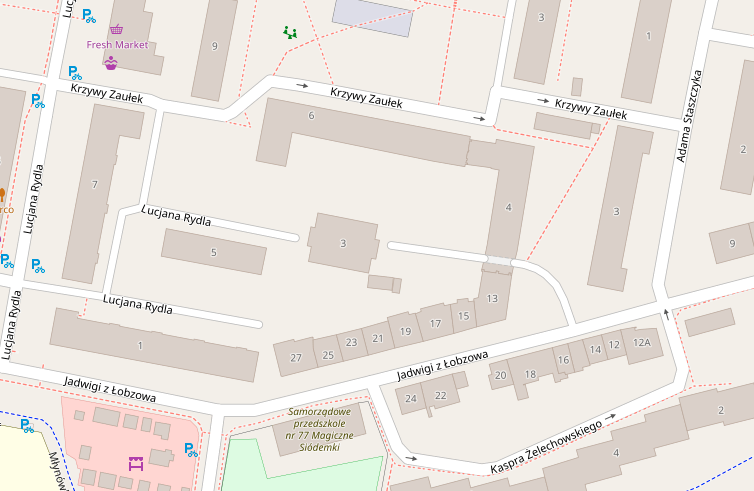
\includegraphics[width=1\textwidth]{img/grafRzecz/osm1}
	\caption[]{Fragment mapy Krakowa\footnotemark.}
	\label{osm1}
\end{figure}

\footnotetext{Zrzut ekranu z strony \href{https://www.openstreetmap.org/}{https://www.openstreetmap.org/}}

Fragment programu przetwarzający mapę z rysunku \ref{osm1} formuje graf, którego krawędzie odpowiadają ulicom, a wierzchołki reprezentują zarówno budynki, jak i istotne elementy dróg: skrzyżowania i strategiczne punkty trasy, które to potrzebne są do idealnego przeprowadzenia ulicy, czyli uwzględnienia zakrętów lub nieliniowych fragmentów drogi.

\captionsetup{justification=centering}
\begin{figure}[htb]
	\centering
	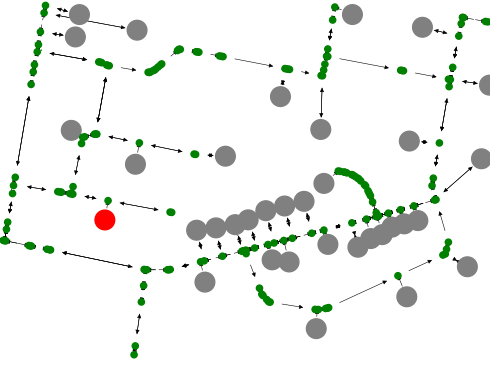
\includegraphics[width=1\textwidth]{img/grafRzecz/osm1Graf}
	\caption[]{Graf rzeczywisty(mieszany) stworzony z mapy z rysunku \ref{osm1}, gdzie czerwone węzeł oznaczają początek trasy listonosza, szare są budynkami mieszkalnymi, zielone to fragmenty ulicy zachowane w celu odwzorowania rzeczywistego jej przebiegu tj. zakrętów, skrzyżowań. Kierunki ulic rzeczywistych (jedno- lub dwukierunkowe drogi) mają wpływ na obecność i kierunek krawędzi.}
	\label{osm1G}
\end{figure}

Program odpowiedzialny za generowanie grafu przy pobieraniu danych z bazy OpenStreetMap filtruje odpowiednie informacje o obiektach i znajduje placówkę pocztową (o ile taka istnieje na danych fragmencie miasta) dzięki konkretnym tagom$^{\cite{osmPropertis}}$. W przypadku wgrania fragmentu mapy, gdzie nie ma poczty, obierany jest inny punkt początkowy trasy listonosza, czy sprzedawcy, który losowany jest wśród istniejących na planie budynków.

Wierzchołki w grafie umieszczono na rysunku odwzorowując rzeczywiste położenie na mapie, przez co krawędzie stworzone na drogach, czy pomiędzy ulicami a budynkami mają odpowiednio proporcjonalne długości. Węzły oznaczono różnymi kolorami, w celu zwiększenia czytelności. Placówkę pocztową lub punkt startowy przedstawiono na czerwono, zwykłe budynki mieszkalne na szaro. Natomiast wierzchołki będące fragmentami drogi pokolorowano na zielono i zmniejszono ich rozmiar względem pozostałych.

Analizując kierunki dróg na rysunku \ref{osm1} można zauważyć, że wpływają one na budowę grafu rzeczywistego z rysunku \ref{osm1G}, który w przypadku kiedy listonosz porusza się np. samochodem jest grafem mieszanym. Niektóre z krawędzi mogą być słabo widoczne, ze względu na duże zagęszczenie węzłów.


\subsubsection{Implementacja grafu rzeczywistego}
\indent\par
Graf rzeczywisty stworzony został  jako obiekt klasy \textit{OsmGraph} przy pomocy funkcji z \textit{OsmParser}, która to odpowiedzialna była za poprawne przetworzenie łańcucha znaków danych w formacie XML$^{\cite{xml}}$.

Dane pobierane z strony internetowej OpenStreetMap za pomocą algorytmu \ref{getData}.
\begin{algorithm}[caption={\textit{getOsmData} funkcja pobierająca dane z strony \textit{opensteermap.org} w formacie \textit{osm}, dla zadanych jej początkowych wartości szerokości i długości geograficznych, tworzących prostokątny obszar do wygenerowania danych.}, label={getData}]
  def getOsmData(top, right, bottom, left):
	  request = "http://api.openstreetmap.org/api/0.6/map?bbox=%f,%f,%f,%f" 
	  						% (left, bottom, right, top)
	  fp = urllib.request.urlopen(request)
	  return fp.read().decode('utf-8') 
\end{algorithm}

Zaimplementowane zostało to tak, żeby główna klasa odpowiedzialna za przechowywanie danych w formacie grafu, na którym mogłyby być wykonywanie algorytmy szukające cykli Eulera, czyli \textit{OsmGraph}, posiadała obiekt \textit{MultiDiGraph} z biblioteki \textit{Networkx}. Wszystkie funkcje z tej klasy operują na nim, odpowiednio modyfikując jego strukturę przy dostosowaniu go rzeczywistości.

Przy przetwarzaniu danych z XML wykorzystano dwie pomocnicze struktury $OsmNode$ i $OsmWay$, odpowiedzialne za przechowanie podstawowych informacji wyciągniętych z bazy OSM.\\
\begin{algorithm}[caption={\textit{OsmNode} struktura tagu XML - $node$, w którym przechowywane są punkty }, label={OsmNode}]
class OsmNode(object):
	def __init__(self, id, x, y):
		self.id = id
		self.x = x
		self.y = y
		self.tags = {}
\end{algorithm}

\begin{algorithm}[caption={\textit{OsmWay} struktura tagu XML - $node$, w którym przechowywane są punkty.}, label={OsmWay}]
	class OsmWay(object):
		def __init__(self, id, osm):
			self.id = id
			self.osm = osm
			self.nds = []  # list of nodes' references
			self.tags = {}
\end{algorithm}

Kolejne elementy zaimplementowane do stworzenia grafu rzeczywistego:
\begin{enumerate}
	\item Pobranie danych przy pomocy klasy \textit{OsmParser}, które przechowywane są w listach jako obiekty typu alg. \ref{OsmNode} i alg. \ref{OsmWay}.   
	\item Wyszukanie budynku z listy $OsmWay$ i $OsmNode$, który w swoich tagach zawiera informację, czy jest to placówka pocztowa. Ewentualne losowe wybranie punktu startowego wśród budynków.
	\item Dodanie budynków mieszkalnych jako wierzchołków grafu.
	\item Wyznaczenie potencjalnych ulic posługując się obiektami typu $OsmNode$ przechowywanymi jako referencje w polu klasy $OsmWay$ \textit{nds} oraz podstawowego równania na prostą o dwóch zadanych punktach (kolejnych referencjach z listy).
	\item Połączenie budynków i potencjalnych punktów ulic, obliczając minimalne odległości wykorzystując funkcję z algorytmu \ref{getDistance}.
	\item Wykonanie funkcji modyfikującej do grafu Eulera opisanej w punkcie \ref{modSkier}. W przypadku, kiedy obszar zaznaczony jest niemożliwy do konwersji(część ulicy jednokierunkowej urwanej na krawędzi), program kończy działanie z informacją, że dla tego fragmentu mapy nie jest w stanie wyznaczyć pożądanej ścieżki.
\end{enumerate}



Odległości pomiędzy budynkami zostały zachowane jako wartości wag odpowiednich krawędzi. Ponieważ pobrano informacje o położeniu geograficznym wskazanych budynków na globie, wykorzystano funkcję Haversine$^{\cite{haver}}$, do wyznaczenia dystansu (równania \ref{haversie} - \ref{haversieD}) między nimi. Określa ona najkrótszą odległość po ortodromie pomiędzy dowolnymi punktami na globie, dzięki ich współrzędnym geograficznym.

\begin{equation} \label{haversie}
	a = \sqrt{sin^2({{\Delta\phi}\over{2}}) + cos(\phi_1) \cdot cos(\phi_2) \cdot sin^2({{\Delta\lambda}\over{2}})}
\end{equation}
\begin{equation} \label{haversieC}
	c = 2 \cdot asin(\sqrt{a})
\end{equation}
\begin{equation} \label{haversieD}
	d = R \cdot c
\end{equation}

\begin{algorithm}[caption={\textit{getDistance} funkcja obliczająca odległości między rzeczywistymi budynkami, generująca wagi dla krawędzi. Przy jej implementacji sugerowano się wzorami \ref{haversie} -  \ref{haversieD}.}, label={getDistance}]
def getDistance(x1, y1, x2, y2):
	x1, y1, x2, y2 = map(radians, [x1, y1, x2, y2])
	dx = x2 - x1
	dy = y2 - y1
	a = sin(dy / 2) ** 2 + cos(y1) * cos(y2) * sin(dx / 2) ** 2
	c = 2 * asin(sqrt(a))
	r = 6371
	r *= 1000	#metres
	return c * r
\end{algorithm}


\newpage
\subsection{Algorytm Fleury’ego} \label{FleuryAlgo}
\indent\par
	Jednym z prostszych sposobów znajdowania cyklu Eulera w UG jest algorytm Fleury'ego. Przede wszystkim zakłada on, że graf, który przyjmuje jest eulerowski, co zapewnia algorytm \ref{makeeulerianUG}. 
\begin{algorithm}[caption={\textit{FleuryAlgorithm} wyszukujący ścieżkę w grafie nieskierowanym}, label={FleuryAlgorithm}]
	def FleuryAlgorithm(graph, startNode):
	adjList = GraphHelper.getAdjList(graph)
	EulerCycle = list()
	
	findNextNode(adjList, startNode, EulerCycle)
	return EulerCycle
\end{algorithm}	
	UG, na którym wywołujemy \textit{FleuryAlgorithm} konwertowany przez prostą funkcję \textit{getAdjList} do listy sąsiedztwa, czyli jednej z możliwych reprezentacji grafu. Wierzchołek startowy, narzucony przez parametr wejściowy, jest tym od którego zaczynane jest poszukiwanie ścieżki. Algorytm odwiedza kolejne krawędzie i usuwa je odkładając kolejno na listę, kierując się zasadą, że połączenie będące mostem (czyli taką krawędzią w grafie, której usunięcie zwiększy ilość jego spójnych składowych SS\footnote{ Jako spójną składową określamy taki podgraf grafu, który jesteśmy w stanie wyodrębnić z całości bez usuwania krawędzi}) usuwane jest w ostateczności. Program działa, aż do odwiedzenia wszystkich krawędzi, a cykl Eulera, będącym rozwiązaniem algorytmu, jest listą kolejno odwiedzonych wierzchołków.

\begin{algorithm}[caption={\textit{findNextNode} rekurencyjna funkcja pomocnicza dla \textit{FleuryAlgorithm} }, label={findNextNode}]
	def findNextNode(adjList, n, EulerCycle):
	EulerCycle.append(n)
	for v in adjList[n]:
	if isBridge(adjList, n, v):
	removeEdge(adjList, n, v)
	findNextNode(adjList, v, EulerCycle)
\end{algorithm}


	Implementacja problemu w pracy została podzielona na 3 główne funkcje: \textit{FleuryAlgorithm} przedstawiony jako nr \ref{FleuryAlgorithm}, który wywołuje rekurencyjną część oznaczoną jako algorytm \ref{findNextNode} oraz fragment sprawdzający, czy aktualnie sprawdzana krawędź jest mostem (alg. \ref{isBridge}).
 
	W algorytmie \ref{isBridge}, w przypadku gdy ilość sąsiadów jest większa niż jeden, program najpierw posiłkuje się prostym algorytmem rekurencyjnym $DFS$ (przeszukiwanie w głąb$^{\cite{cormen}}$), który ma za zadanie wyznaczyć ilość spójnych składowych. Następnie usuwana jest sprawdzana krawędź i ponownie obliczana jest ilość SS. Finalnie przywraca się wcześniej wspomniane połączenie między-wierzchołkowe. W zależności, od tego czy wartości obliczone są różne zwracana jest zmienna typu $Bool$, pozwalająca lub nie na poszukiwanie kolejnego wierzchołka w funkcji \textit{findNextNode}.
	
	Złożoność obliczeniowa szacowana jest na $O(V(V+E))$ \label{zl_Fle}.

\begin{algorithm}[caption={\textit{isBridge} rekurencyjna funkcja pomocnicza dla \textit{FleuryAlgorithm} }, label={isBridge}]
def isBridge(adjList, u, v):
	if len(adjList[u]) == 1:
		return True
	else:
		listOfVisitedNeighbours = [False] * len(adjList)
		cntBeforeRestoreEdge = DFS(adjList, u, listOfVisitedNeighbours)
		
		removeEdge(adjList, u, v)
		listOfVisitedNeighbours = [False] * len(adjList)
		cntAfterRestoreEdge = DFS(adjList, u, listOfVisitedNeighbours)
		
		# restore edge
		addEdge(adjList, u, v)
		
		return cntBeforeRestoreEdge < cntAfterRestoreEdge

\end{algorithm}

\subsubsection{Wizualizacja grafu nieskierowanego}
\indent\par
Działanie algorytmu opisanego w rozdziale \ref{FleuryAlgo} zaprezentowano na podstawie grafu z rysunku \ref{f_DD}. Jest to sieć o modelu Barabási–Alberta, jednak aby zaimplementowany program zadziałał poprawnie wymagane było spełnienie twierdzenia \ref{twEuleraUG}. Stworzony przy pomocy algorytmu \ref{makeeulerianUG}, nowy graf, który bazował na wspomnianym modelu BA, zaprezentowano na rysunku \ref{f_DDD}. 

Na rysunkach \ref{imgFluAlgoEgz1} i \ref{imgFluAlgoEgz2} przedstawiono kolejne kroki  cyklu Eulera wygenerowanego przez algorytm \ref{FleuryAlgorithm} na grafie \ref{f_DDD}.
	\begin{figure}[!p]
			\centering
		\subfloat[Sieć złożona o modelu Barabási–Alberta.]{\label{f_DD}
			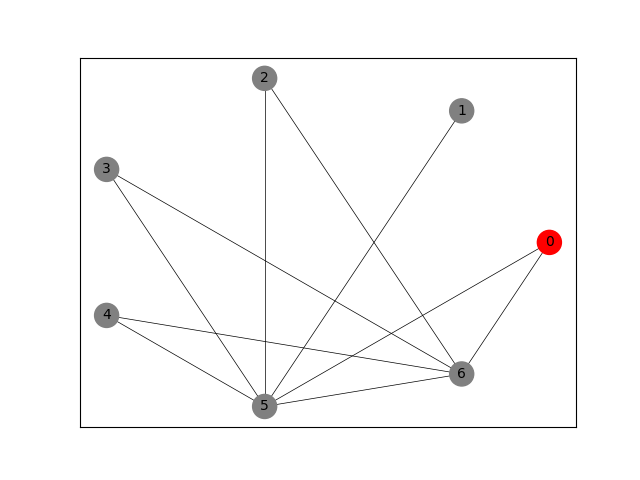
\includegraphics[width=0.7\textwidth]{img/fluAlgo/flu_algo99.png}}		\quad
		\subfloat[Graf stworzony na podstawie sieci o modelu Barabási–Alberta, przetworzonej przez funkcję \textit{makeEulerianGraph}.]{\label{f_DDD}
			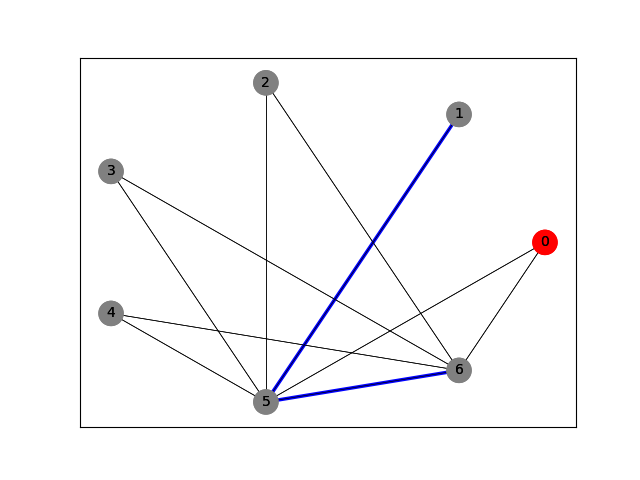
\includegraphics[width=0.7\textwidth]{img/fluAlgo/flu_algo0.png}}
		
		\caption[]{Sieć złożona o modelu Barabási–Alberta (rozdział \ref{BarabasiAlbert}), dla parametrów $m_0=5, t=7$ na rysunku \ref{f_DD}. Ta sama sieć po modyfikacji do grafu Eulera na rysunku \ref{f_DDD}, na niebiesko zaznaczono krawędzie wielokrotne,w tym przypadku są to połączenia pomiędzy wierzchołkami (1, 5) i (5, 6), stworzone sztucznie algorytmem \ref{makeeulerianUG}. Czerwony wierzchołek jest punktem startowym wyznaczania cyklu.}
		\label{f_graph}
	\end{figure}	
	\captionsetup{justification=centering}
	
	\begin{figure}[!p]
		\centering
		\subfloat[Krok 1: 0 -> 5]{\label{f_a}
			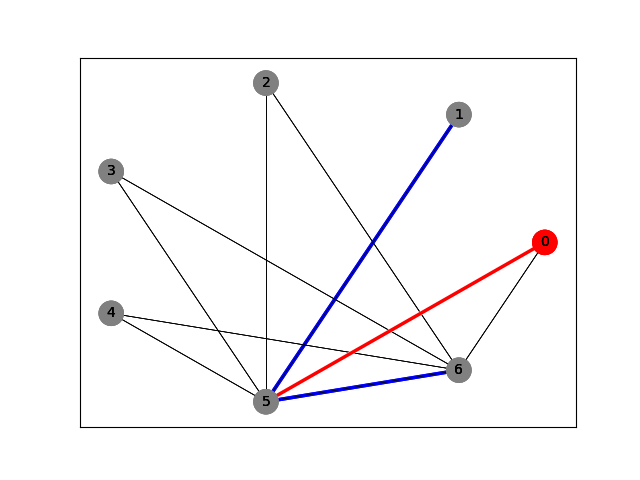
\includegraphics[width=0.45\textwidth]{img/fluAlgo/flu_algo1.png}}
		\quad
		\subfloat[Krok 2: 5 -> 1]{\label{f_b}
			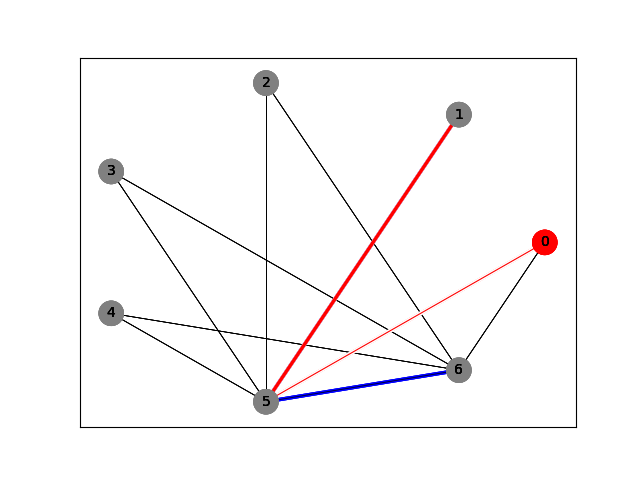
\includegraphics[width=0.45\textwidth]{img/fluAlgo/flu_algo2.png}}
		\quad
		\subfloat[Krok 3: 1 -> 5]{\label{f_c}
			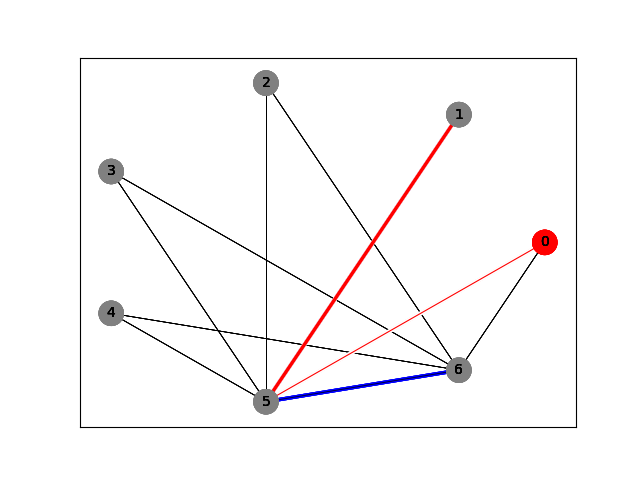
\includegraphics[width=0.45\textwidth]{img/fluAlgo/flu_algo3.png}}
		\quad
		\subfloat[Krok 4: 5 -> 2]{\label{f_d}
			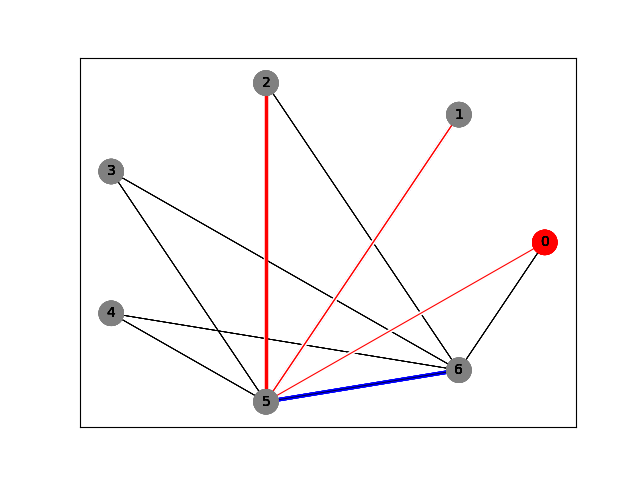
\includegraphics[width=0.45\textwidth]{img/fluAlgo/flu_algo4.png}}
		\quad
		\subfloat[Krok 5: 2 -> 6]{\label{f_e}
			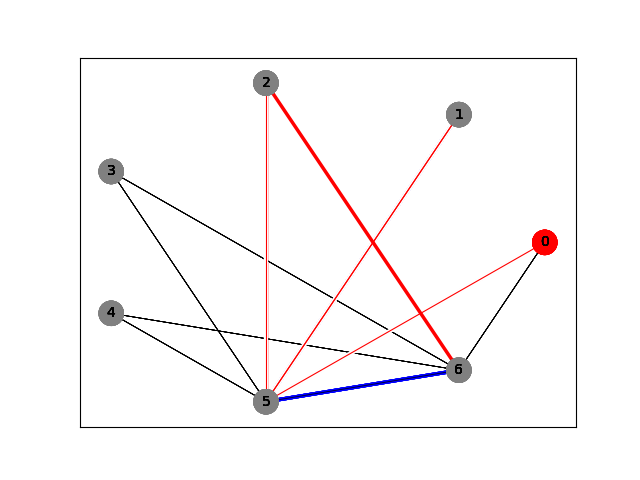
\includegraphics[width=0.45\textwidth]{img/fluAlgo/flu_algo5.png}}
		\quad
		\subfloat[Krok 6: 6 -> 4]{\label{f_f}
			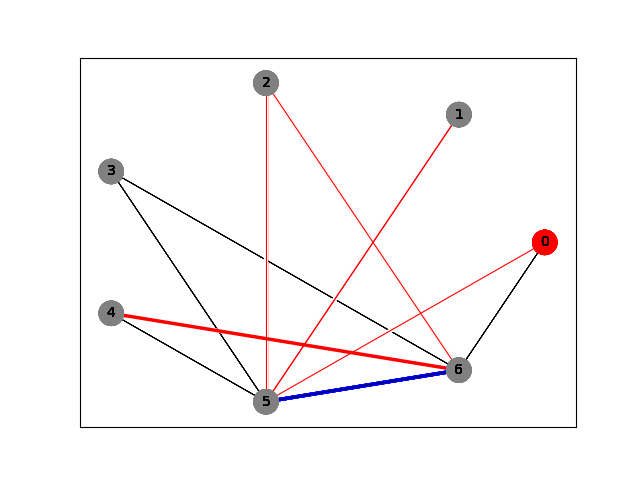
\includegraphics[width=0.45\textwidth]{img/fluAlgo/flu_algo6.png}}
		
		\caption[]{Pierwsze 6 kroków algorytmu Fleury'ego na grafie z rysunku \ref{f_DDD}. Grubą linią czerwoną oznaczono aktualną krawędź cyklu, cieńszą krawędzie już odwiedzone, a na niebiesko krawędzie wielokrotne, wynikające z funkcji \textit{makeEulerianGraph}. Cały cykl Eulera przebiega kolejno przez wierzchołki: 0, 5, 1, 5, 2, 6, 4, 5, 3, 6, 5, 6, 0.}
		\label{imgFluAlgoEgz1}
	\end{figure}	
	
	\begin{figure}[!p]
		\centering
		\subfloat[Krok 7: 4 -> 5]{\label{f_g}
			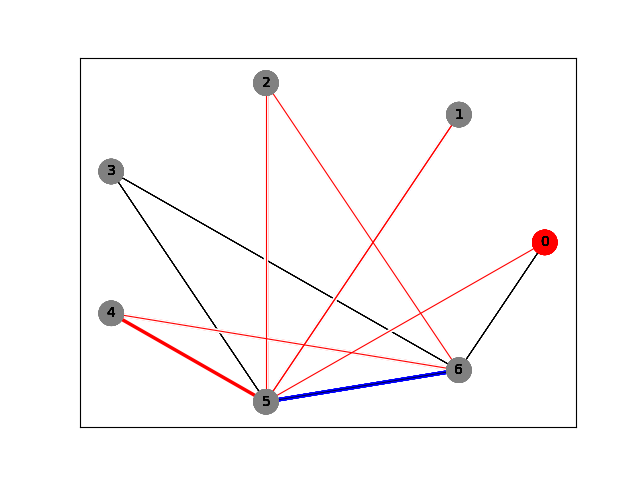
\includegraphics[width=0.45\textwidth]{img/fluAlgo/flu_algo7.png}}
		\quad
		\subfloat[Krok 8: 5 -> 3]{\label{f_h}
			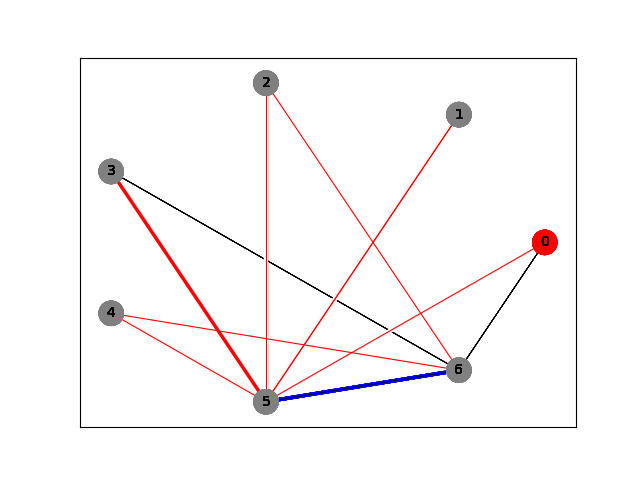
\includegraphics[width=0.45\textwidth]{img/fluAlgo/flu_algo8.png}}
		\quad
		\subfloat[Krok 9: 3 -> 6]{\label{f_i}
			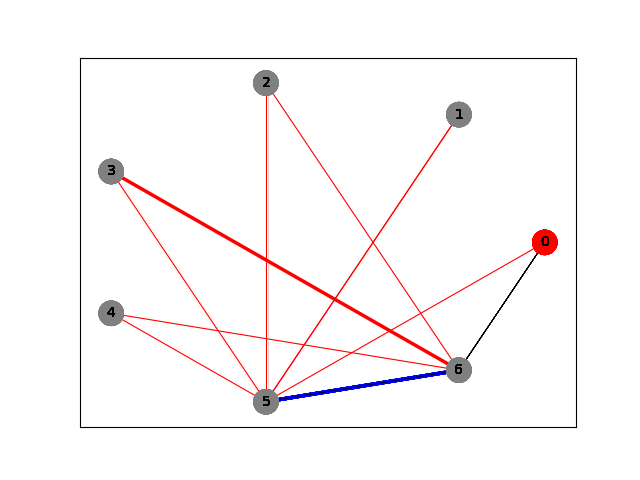
\includegraphics[width=0.45\textwidth]{img/fluAlgo/flu_algo9.png}}
		\quad
		\subfloat[Krok 10: 6 -> 5]{\label{f_j}
			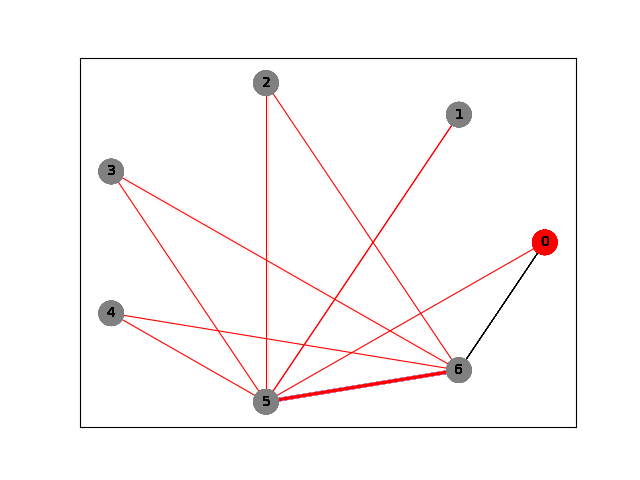
\includegraphics[width=0.45\textwidth]{img/fluAlgo/flu_algo10.png}}
		\quad
		\subfloat[Krok 11: 5 -> 6]{\label{f_k}
			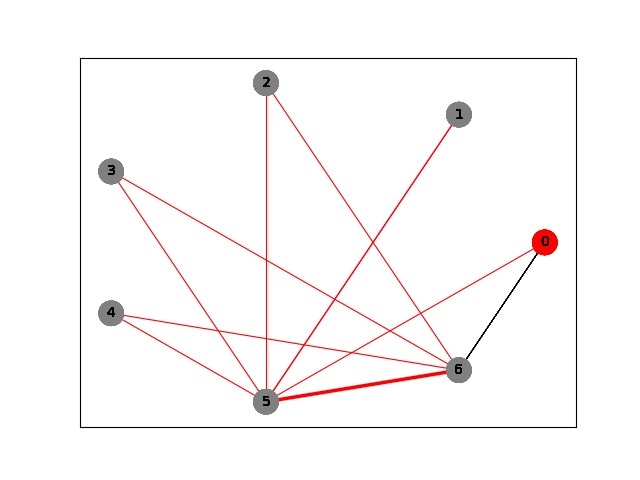
\includegraphics[width=0.45\textwidth]{img/fluAlgo/flu_algo11.png}}
		\quad
		\subfloat[Krok 12: 6 -> 0]{\label{f_l}
			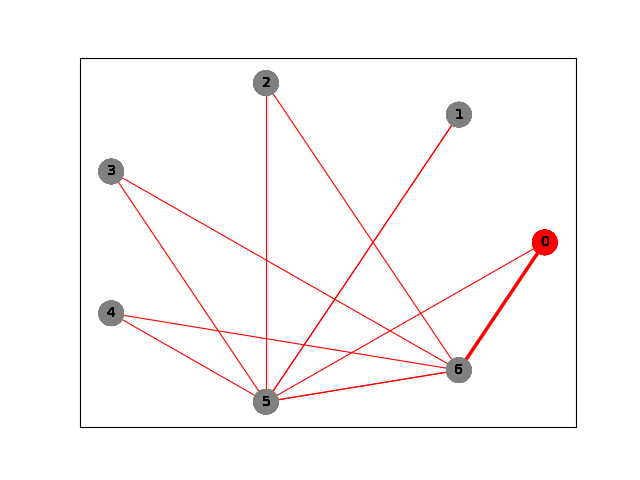
\includegraphics[width=0.45\textwidth]{img/fluAlgo/flu_algo12.png}}
		
		\caption[]{Kontynuacja rysunku \ref{imgFluAlgoEgz1}. Kolejne 6 kroków algorytmu Fleury'ego na grafie z rysunku \ref{f_DDD}, które kończą pełny cykl Eulera. Grubą linią czerwoną oznaczono aktualną krawędź cyklu, cieńszą krawędzie już odwiedzone, a na niebiesko krawędzie wielokrotne, wynikające z funkcji \textit{makeEulerianGraph}. Cały  cykl Eulera przebiega kolejno przez wierzchołki: 0, 5, 1, 5, 2, 6, 4, 5, 3, 6, 5, 6, 0.}
		\label{imgFluAlgoEgz2}
	\end{figure}


\subsection{Algorytm Hierholzera} \label{hier}
\indent\par
	Kolejnym zaimplementowanym sposobem znajdowania cyklu Eulera w UG i DG jest algorytm Hierholzera$^{\cite{hierholzer}}$. Tak jak dla algorytmu opisanego w \ref{FleuryAlgo} wymagane jest, żeby graf był eulerowski, co w tym przypadku mogą zapewnić algorytmy \ref{makeeulerianUG} i \ref{makeeulerianDG}, w zależności od wartości zmiennej \textit{isDirected}.
	
	Podobnie jak algorytm z rozdziału \ref{FleuryAlgo}, operuje on na liście sąsiedztwa, co było najbardziej efektywnym wyborem zważywszy na typy danych testowanych (sieci opisane w \ref{SieciZlozone}). Wierzchołek startowy znany jest z góry. Poszukiwana od niego zaczęte polegają na znajdowaniu mniejszych cykli (domkniętych szlaków) usuwając przy tym przebyte krawędzie. Wykorzystuje się przy tym stos, na który w odpowiedniej kolejności odkłada się odwiedzone wierzchołki.
	
\captionsetup{justification=centering}
\begin{algorithm}[caption={\textit{HierholzerAlgorithm} funkcja wyznaczająca ścieżkę dla grafów skierowanych i nieskierowanych }, label={HierholzerAlgorithm}]
def HierholzerAlgorithm(graph, isDirected, startNode):
	adjList = GraphHelper.getAdjList(graph)
	EulerCycle = list()
	stackOfNodes = deque()
	
	node = startNode
	EulerCycle.append(node)
	
	while True:
		if checkOutDegree(adjList, node):
			v = getNextOutEdge(adjList, node)
			stackOfNodes.append(node)
			removeEdge(adjList, node, v, isDirected)
			node = v
		else:
			node = stackOfNodes.pop()
			EulerCycle.append(node)
		
		if not stackOfNodes:
			break
		
	EulerCycle.reverse()
	return EulerCycle
\end{algorithm}

	Złożoność obliczeniowa szacowana jest na $O(E)$. \label{zl_H}
	
\subsubsection{Wizualizacja grafu nieskierowanego}
\indent\par
	Na rysunkach \ref{imgHierAlgoEgz1} i \ref{imgHierAlgoEgz2} zilustrowano przebieg algorytmu z rozdziału \ref{hier} dla grafu nieskierowanego o modelu sieci \textit{small-world} (rys. \ref{h_graph}). Przed wykonaniem programu sprawdzono stworzoną sieć Wattsa–Strogatza pod kątem spełnienia warunków koniecznych do miana grafu Eulera (tw. \ref{twEuleraUG}). Ponieważ parzysta ilość krawędzi przy każdym z wierzchołków była zachowana, niewymagane były dalsze modyfikacje, więc algorytm przeszukiwał pierwotnie stworzony graf.
	
	\begin{figure}[!htb]
		\centering
		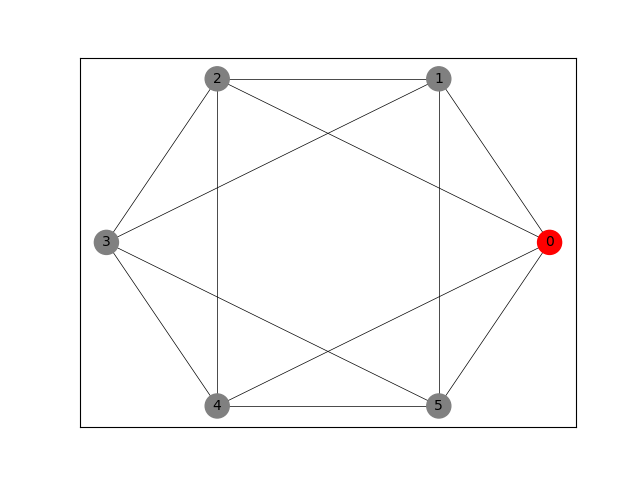
\includegraphics[width=1\textwidth]{img/heiAlgo/hei_algo0.png}
		\caption[]{Sieć złożona o modelu  Wattsa–Strogatza (rozdział \ref{WSWS}), dla parametrów $n=6, k=4, p=0$. Wierzchołek początkowy zaznaczono kolorem czerwonym.}
		\label{h_graph}
	\end{figure}	

	\captionsetup{justification=centering}
	\begin{figure}[!p]
		\centering
		\subfloat[Krok 1: 0 -> 1]{\label{h_b}
			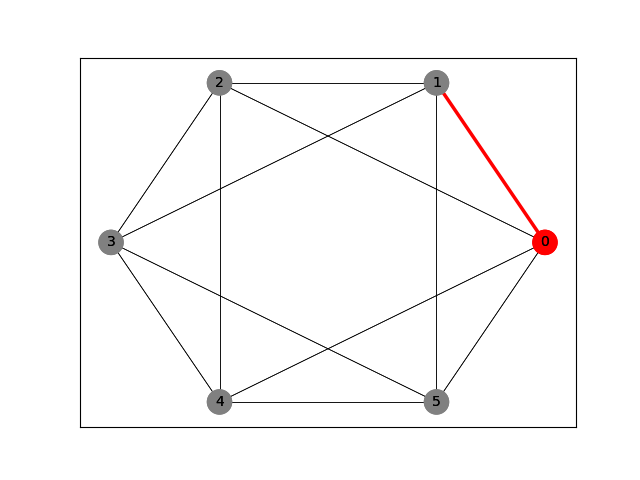
\includegraphics[width=0.47\textwidth]{img/heiAlgo/hei_algo1.png}}
		\quad
		\subfloat[Krok 2: 1 -> 2]{\label{h_c}
			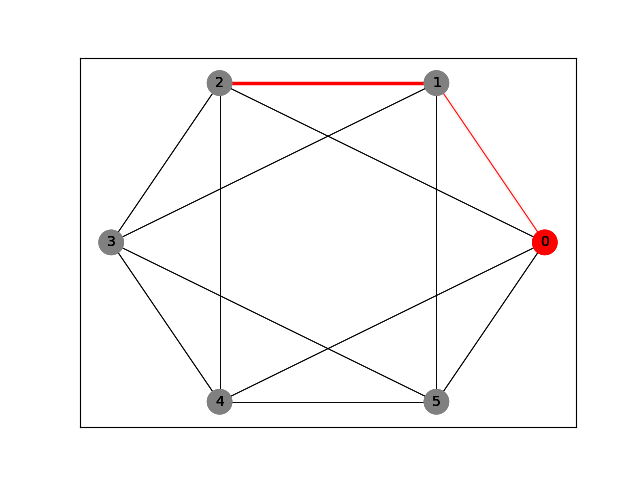
\includegraphics[width=0.47\textwidth]{img/heiAlgo/hei_algo2.png}}
		\quad
		\subfloat[Krok 3: 2 -> 0]{\label{h_d}
			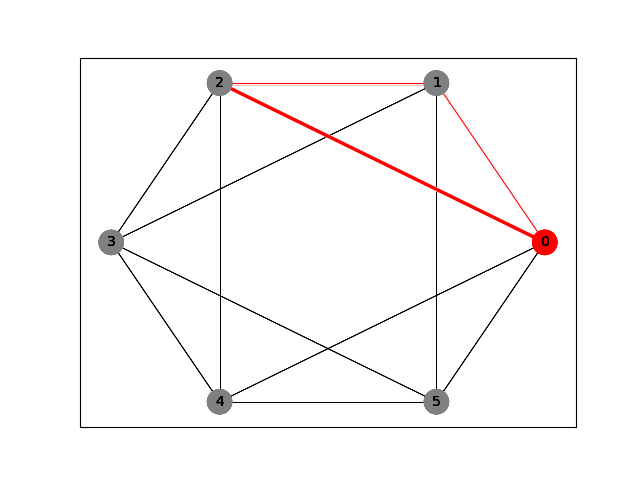
\includegraphics[width=0.47\textwidth]{img/heiAlgo/hei_algo3.png}}
		\quad
		\subfloat[Krok 4: 0 -> 5]{\label{h_e}
			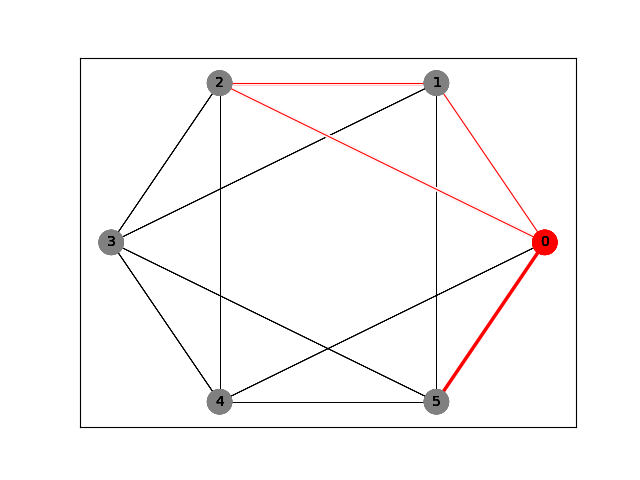
\includegraphics[width=0.47\textwidth]{img/heiAlgo/hei_algo4.png}}
		\quad
		\subfloat[Krok 5: 5 -> 1]{\label{h_f}
			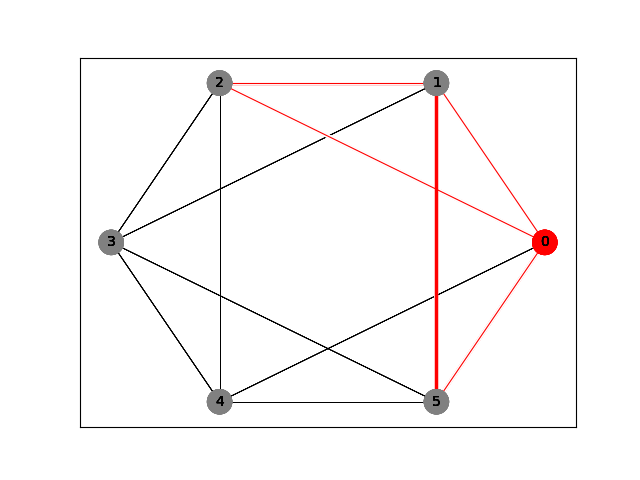
\includegraphics[width=0.47\textwidth]{img/heiAlgo/hei_algo5.png}}
		\quad
		\subfloat[Krok 6: 1 -> 3]{\label{h_g}
			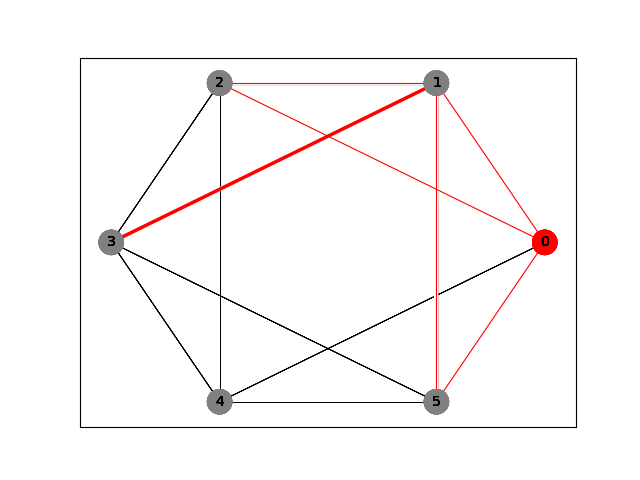
\includegraphics[width=0.47\textwidth]{img/heiAlgo/hei_algo6.png}}
		\caption[]{Pierwsze 6 kroków algorytmu Hierholzera na nieskierowanym grafie wejściowym z rysunku \ref{h_graph}. Grubą linią czerwoną oznaczono aktualną krawędź, cieńszą krawędzie już odwiedzone. Cały cykl Eulera przebiega kolejno przez wierzchołki: 0, 1, 2, 0 , 5, 1, 3, 2, 4, 3, 5, 4, 0.}
		\label{imgHierAlgoEgz1}
	\end{figure}	
	
	\begin{figure}[!p]
		\centering		
		\subfloat[Krok 7: 3 -> 2]{\label{h_h}
			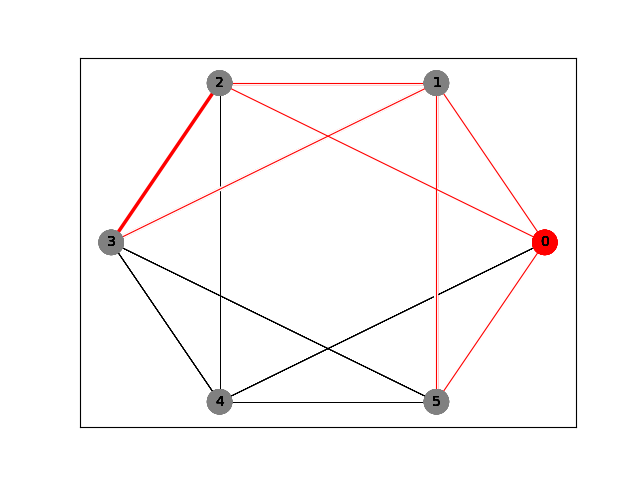
\includegraphics[width=0.47\textwidth]{img/heiAlgo/hei_algo7.png}}
		\quad
		\subfloat[Krok 8: 2 -> 4]{\label{h_i}
			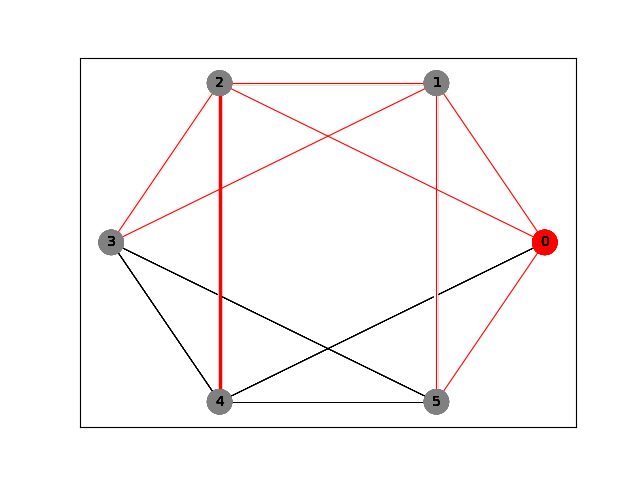
\includegraphics[width=0.47\textwidth]{img/heiAlgo/hei_algo8.png}}
		\quad
		\subfloat[Krok 9: 4 -> 3]{\label{h_j}
			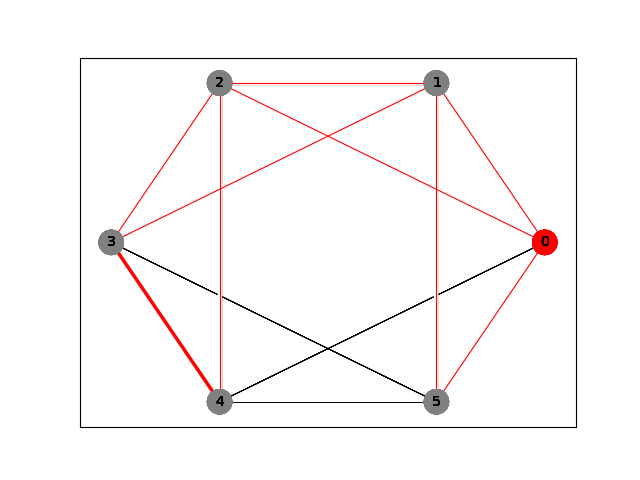
\includegraphics[width=0.47\textwidth]{img/heiAlgo/hei_algo9.png}}
		\quad
		\subfloat[Krok 10: 3 -> 5]{\label{h_k}
			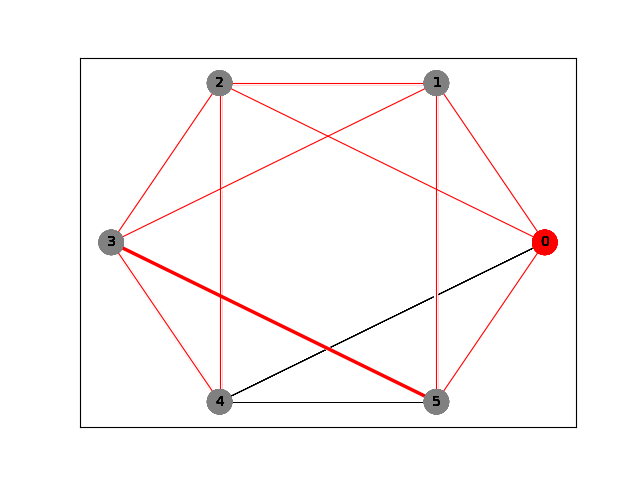
\includegraphics[width=0.47\textwidth]{img/heiAlgo/hei_algo10.png}}
		\quad	
		\subfloat[Krok 11: 5 -> 4]{\label{h_l}
			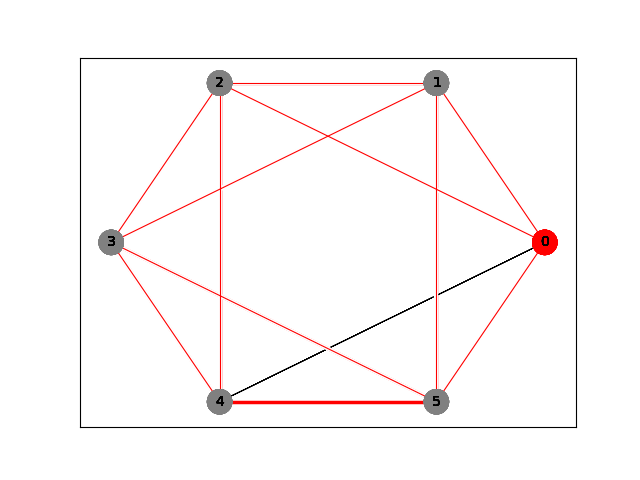
\includegraphics[width=0.47\textwidth]{img/heiAlgo/hei_algo11.png}}
		\quad
		\subfloat[Krok 12: 4 -> 0]{\label{h_m}
			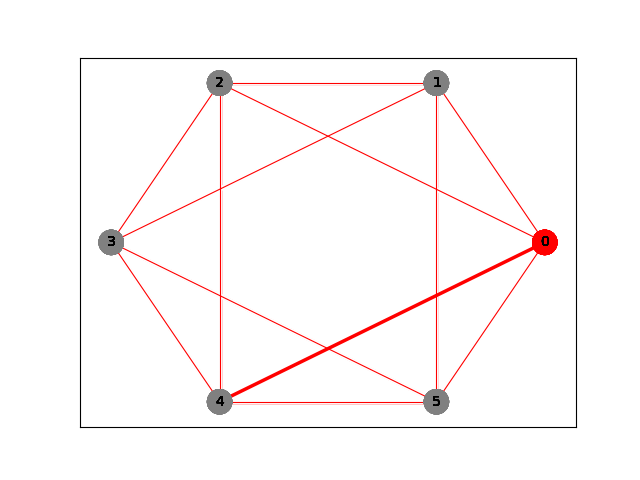
\includegraphics[width=0.47\textwidth]{img/heiAlgo/hei_algo12.png}}
		
		\caption[]{Kontynuacja rysunku \ref{imgHierAlgoEgz1}. Kolejne 6 kroków algorytmu Hierholzera na nieskierowanym grafie wejściowym z rysunku \ref{h_graph}, znajdujących pełen cykl. Grubą linią czerwoną oznaczono aktualną krawędź, cieńszą krawędzie już odwiedzone. Cały cykl Eulera przebiega kolejno przez wierzchołki: 0, 1, 2, 0 , 5, 1, 3, 2, 4, 3, 5, 4, 0.}
		\label{imgHierAlgoEgz2}
	\end{figure}
\newpage
\subsubsection{Wizualizacja grafu skierowanego}
\indent\par
	Algorytm zilustrowano również dla losowego grafu skierowanego z rysunku \ref{h_DD}, który został stworzony przy pomocy funkcji \textit{fast\_gnp\_random\_graph} z biblioteki \textit{Networkx}. 
	
	Należy zwrócić uwagę na działanie funkcji modyfikującej do postaci eulerowskiej (opisanej w \ref{modSkier}). Początkowo stworzony graf nie spełniał warunków twierdzenia \ref{twEuleraDG}, dlatego wymagana była jego konwersja przy pomocy algorytmu \ref{makeeulerianDG}. Nowo powstały DG zaprezentowano na rysunku \ref{h_DDD}, gdzie niebieski kolor symbolizuje sztuczne dodane krawędzie wielokrotne. W tym przypadku są to [2, 0], [3, 1] i [4, 3], stabilizujące różnicę wejść i wyjść z każdego wierzchołka.
	
	Przebieg kolejnych kroków pomiędzy wierzchołkami można zaobserwować na rysunkach \ref{imgHierAlgoEgz3}, \ref{imgHierAlgoEgz4} i \ref{imgHierAlgoEgz5}.
	
	\captionsetup{justification=centering}	
	\begin{figure}[!p]
		\centering
		\subfloat[Losowy graf skierowany.]{\label{h_DD}
			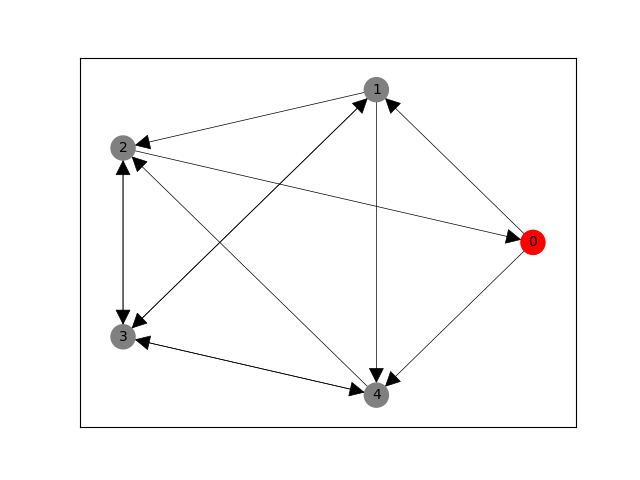
\includegraphics[width=0.69\textwidth]{img/heiAlgo/DIRhei_algo99.png}}		\quad
		\subfloat[Graf skierowany po modyfikacjach algorytmu \textit{makeEulerianDiGraph} do postaci grafu eulerowskiego.]{\label{h_DDD}
			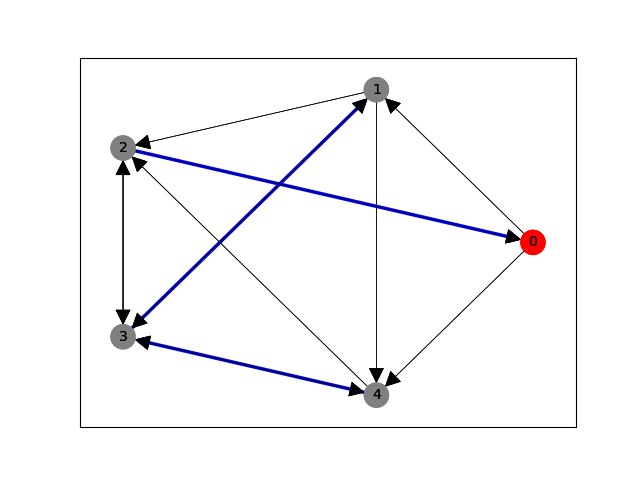
\includegraphics[width=0.69\textwidth]{img/heiAlgo/DIRhei_algo0.png}}
		
		\caption[]{Losowy graf skierowany stworzony przy pomocy funkcji \textit{fast\_gnp\_random\_graph} o parametrach $n=5, p=0.5$, gdzie $n$ - ilość wierzchołków, a $p$ - prawdopodobieństwo utworzenia krawędzi na rysunku \ref{h_DD}. Ten sam graf po modyfikacji do grafu Eulera na rysunku \ref{h_DDD}, na niebiesko zaznaczono krawędzie wielokrotne, stworzone sztucznie algorytmem nr \ref{makeeulerianDG}, są to [2, 0], [3, 1] i [4, 3]. Czerwony wierzchołek jest punktem startowym wyznaczania cyklu.}
		\label{h_Dgraph}
	\end{figure}	

   \captionsetup{justification=centering}
   \begin{figure}[!p]
   	\centering
   	\subfloat[Krok 1: 0 -> 1]{\label{hd_a}
   		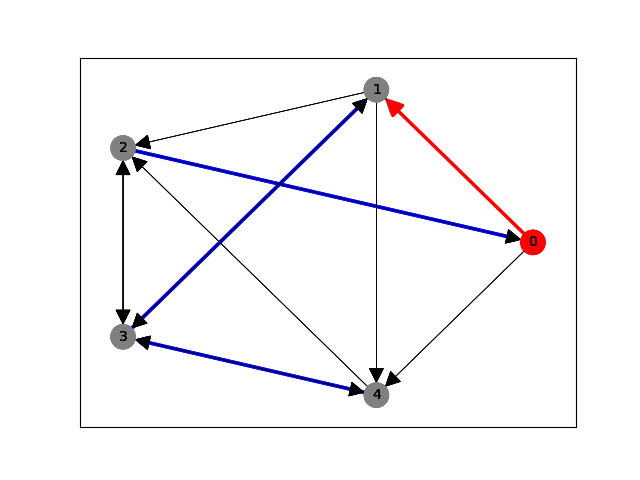
\includegraphics[width=0.47\textwidth]{img/heiAlgo/DIRhei_algo1.png}}
   	\quad
   	\subfloat[Krok 2: 1 -> 2]{\label{hd_b}
   		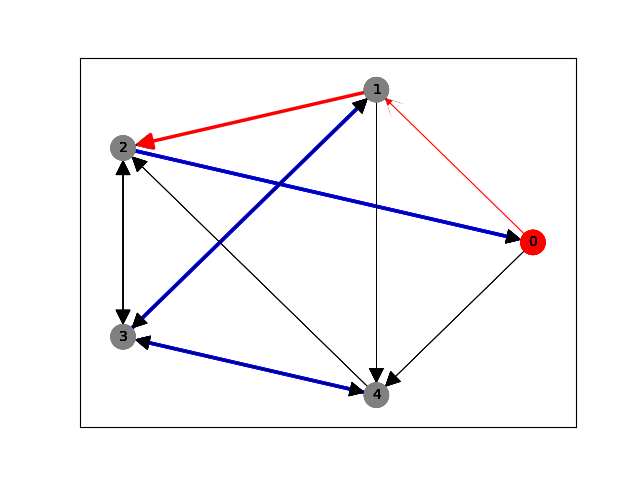
\includegraphics[width=0.47\textwidth]{img/heiAlgo/DIRhei_algo2.png}}
   	\quad
   	\subfloat[Krok 3: 2 -> 0]{\label{hd_c}
   		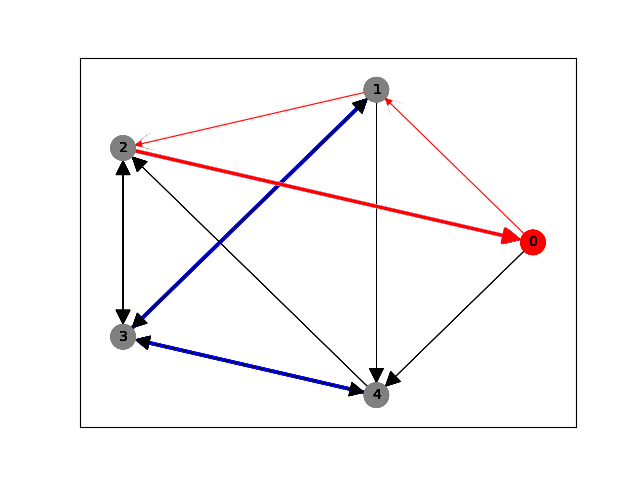
\includegraphics[width=0.47\textwidth]{img/heiAlgo/DIRhei_algo3.png}}
   	\quad
   	\subfloat[Krok 4: 0 -> 4]{\label{hd_d}
   		\includegraphics[width=0.47\textwidth]{img/heiAlgo/DIRhei_algo4.png}}
   	\quad
   	\subfloat[Krok 5: 4 -> 2]{\label{hd_e}
   		\includegraphics[width=0.47\textwidth]{img/heiAlgo/DIRhei_algo5.png}}
   	
   	\caption[]{Kroki 1-5 algorytmu Hierholzera na skierowanym grafie wejściowym z rysunku \ref{h_Dgraph}. Grubą linią czerwoną oznaczono aktualną krawędź, cieńszą krawędzie już odwiedzone, a na niebiesko krawędzie wielokrotne. Cały cykl Eulera przebiega kolejno przez wierzchołki: 0, 1, 2, 0, 4, 2, 3, 1, 3, 1, 4, 3, 4, 3, 2, 0.}
   	\label{imgHierAlgoEgz3}
   \end{figure}	

   \captionsetup{justification=centering}
   \begin{figure}[p]
   	\centering
   	\subfloat[Krok 6: 2 -> 3]{\label{hd_f}
   		\includegraphics[width=0.47\textwidth]{img/heiAlgo/DIRhei_algo6.png}}
   	\quad
   	\subfloat[Krok 7: 3 -> 1]{\label{hd_g}
   		\includegraphics[width=0.47\textwidth]{img/heiAlgo/DIRhei_algo7.png}}
   	\quad
   	\subfloat[Krok 8: 1 -> 3]{\label{hd_h}
   		\includegraphics[width=0.47\textwidth]{img/heiAlgo/DIRhei_algo8.png}}
   	\quad
   	\subfloat[Krok 9: 3 -> 1]{\label{hd_i}
   		\includegraphics[width=0.47\textwidth]{img/heiAlgo/DIRhei_algo9.png}}
   	\quad
   	\subfloat[Krok 10: 1 -> 4]{\label{hd_j}
   		\includegraphics[width=0.47\textwidth]{img/heiAlgo/DIRhei_algo10.png}}
   	
   	\caption[]{Kontynuacja rysunku \ref{imgHierAlgoEgz3}. Kroki 6-10 algorytmu Hierholzera na skierowanym grafie wejściowym z rysunku \ref{h_Dgraph}. Grubą linią czerwoną oznaczono aktualną krawędź, cieńszą krawędzie już odwiedzone, a na niebiesko krawędzie wielokrotne. Cały cykl Eulera przebiega kolejno przez wierzchołki: 0, 1, 2, 0, 4, 2, 3, 1, 3, 1, 4, 3, 4, 3, 2, 0.}
   	\label{imgHierAlgoEgz4}
   \end{figure}	

	\captionsetup{justification=centering}
	\begin{figure}[p]
	\centering
	\subfloat[Krok 11: 4 -> 3]{\label{hd_k}
		\includegraphics[width=0.47\textwidth]{img/heiAlgo/DIRhei_algo11.png}}
	\quad
	\subfloat[Krok 12: 3 -> 4]{\label{hd_l}
		\includegraphics[width=0.47\textwidth]{img/heiAlgo/DIRhei_algo12.png}}
	\quad
	\subfloat[Krok 13: 4 -> 3]{\label{hd_m}
		\includegraphics[width=0.47\textwidth]{img/heiAlgo/DIRhei_algo13.png}}
	\quad
	\subfloat[Krok 14: 3 -> 2]{\label{hd_n}
		\includegraphics[width=0.47\textwidth]{img/heiAlgo/DIRhei_algo14.png}}
	\quad
	\subfloat[Krok 15: 2 -> 0]{\label{hd_o}
		\includegraphics[width=0.47\textwidth]{img/heiAlgo/DIRhei_algo15.png}}
	
	\caption[]{Kontynuacja rysunku \ref{imgHierAlgoEgz4}. Kroki 11-15 algorytmu Hierholzera na skierowanym grafie wejściowym z rysunku \ref{h_Dgraph}. Grubą linią czerwoną oznaczono aktualną krawędź, cieńszą krawędzie już odwiedzone. Cały cykl Eulera przebiega kolejno przez wierzchołki: 0, 1, 2, 0, 4, 2, 3, 1, 3, 1, 4, 3, 4, 3, 2, 0.}
	\label{imgHierAlgoEgz5}
	\end{figure}	
\newpage
% ======================= 4 =======================
\newpage
\section{Wyniki}
\subsection{Generowanie grafów losowych}
\indent\par
Grafy losowe opisane w tym rozdziale generowane są do maksymalnej ilości 2000 wierzchołków. Ograniczona liczba wynika z długiego czasu ich powstawania, co można zauważyć w tabelach \ref{Tab:gen_BA}, \ref{Tab:gen_WS} i \ref{Tab:gen_DiG}. Średnia długość tworzenia dla skrajnego przypadku sięga ponad 11h, a próbek testowych dla każdej ilości węzłów było 5. 

Długi czas wynikał z ilości permutacji wykorzystanych przy tworzeniu grafu Eulera (rozdział \ref{modyfikacja}), które i tak zostały ograniczone. Dla każdego zestawu możliwych par wykorzystywana była funkcja \textit{shortest\_path\_length} z biblioteki \textit{Networkx}. Duże ilości jej wywołań wypłynęły znacznie na wydajność programu.

Podczas generowania sieci złożonych Barabási–Alberta i Wattsa–Strogatza, które są szerzej opisane w rozdziale \ref{SieciZlozone}, zebrano wyniki zaprezentowane odpowiednio w tabelach \ref{Tab:gen_BA} i \ref{Tab:gen_WS}. Parametry, dla których tworzono sieci o modelu BA to $m_0 = w$, $t = {w\over2}$, gdzie $w$ jest liczbą wierzchołków. Przy generowaniu losowych sieci WS, wybrano następujące wielkości: $n = w$, $k = {w\over2}$, $p=0.75$, gdzie $w$ - liczba węzłów.



Porównując wyniki z tabel \ref{Tab:gen_BA} i \ref{Tab:gen_WS} łatwo można zauważyć, że pomimo podobnej ilość krawędzi w grafach, czasy ich generowania (uwzględniające funkcję z rozdziału \ref{mgnieskier}) zaczynają się rozbiegać już w okolicach 100 wierzchołków, na korzyść modelu Barabási–Alberta.

Wyniki z tabeli \ref{Tab:gen_DiG} znacznie różnią się od \ref{Tab:gen_BA} i \ref{Tab:gen_WS}, spowodowane jest to innym typem wejściowym (w tym przypadku jest to DG), a co za tym idzie, funkcja modyfikująca do grafu Eulera jest inna. Warunki twierdzenia o grafie skierowanym (tw. \ref{twEuleraDG}) wpływają na ilość obliczeń możliwych permutacji. 

\begin{figure}[H]
	\centering
	\centering
	\subfloat[Zależność stworzonych krawędzi dla każdego typu grafów testowych w zależności od ilości wierzchołków, gdzie $n$ - liczba wierzchołków, $e$ - liczba krawędzi.]{\label{e_n}
		\includegraphics[angle=270,width=0.85\textwidth]{img/wyniki/E_N}}
	\quad
	\subfloat[Czas generowania grafów, uwzględniając funkcję modyfikującą do grafu Eulera, gdzie $n$ - liczba węzłów, $t$ - czas podany w sekundach.]{\label{gen_n}
		\includegraphics[angle=270,width=0.85\textwidth]{img/wyniki/gen_n}}
	\caption[]{Wykresy porównujące dane z tabel \ref{Tab:gen_BA}, \ref{Tab:gen_WS} i \ref{Tab:gen_DiG}.}
	\label{gen}
\end{figure}


Do generowania skierowanych grafów losowych, których dane zebrano w tabeli \ref{Tab:gen_DiG}, wykorzystano funkcję \textit{fast\_gnp\_random\_graph} z biblioteki \textit{Networkx}, która przyjmuje wartości $n$ i $p$, gdzie $n$ - ilość wierzchołków, $p$ - prawdopodobieństwo stworzenia krawędzi (w przypadku stworzonych danych obrano jego stałą wartość: $p= 0.75$).


Wyniki zgromadzone w tabelach \ref{Tab:gen_BA}, \ref{Tab:gen_WS} i \ref{Tab:gen_DiG} przeniesione zostały na wykresy z rysunków \ref{e_n}, \ref{gen_n}. Na pierwszym z nich można zauważyć znaczą różnicę w ilości krawędzi pomiędzy grafem skierowanym a sieciami złożonymi, natomiast te drugie (modele WS i BA) są sobie bardzo bliskie, ich funkcję nakładają się na siebie. Ma to swoje przełożenie na czas generowania takich grafów (rys. \ref{gen_n}), gdzie funkcja DG rośnie bardzo szybko, z znaczną różnicą względem dwóch pozostałych. Natomiast dla sieci Barabási–Alberta i Wattsa–Strogatza czasy zaczynają się zauważalnie różnić powyżej 1000 wierzchołków.



\subsection{Algorytm Fleury'ego} \label{Fleu_wyniki}
\indent\par
	Wyniki z znajdowania cyklu Eulera dla grafów nieskierowanych przy pomocy algorytmu Fleury'ego zostały zaprezentowane w tabelach \ref{Tab:BA_Fleury} i \ref{Tab:WS_Fleury}. 
	
	Stos w języku Python posiada limit zapobiegający nieskończonej rekurencji i zbyt wielkiemu wykorzystaniu zasobów pamięciowych, co mogłoby skutkować awarią systemu. Ponieważ funkcja ta działa rekurencyjnie, nawet przy zwiększeniu limitu do maksymalnej wartości, wykonano pomiary tylko do 280 węzłów.

	Analizując rysunek \ref{fle_n}, na którym przedstawiono wykresy powstałe z danych z dwóch tabel reprezentujących czasy wykonania algorytmu dla modeli sieci złożonych Barabási–Alberta i Wattsa–Strogatza (tab. \ref{Tab:BA_Fleury}, \ref{Tab:WS_Fleury}), możliwe jest zauważenie, że dla początkowych mniejszych ilości wierzchołków nie ma większej różnicy. Wprowadzając oznaczenie $\Delta t(n) = t_{WattsaStrogatz}(n) - t_{BarabásiAlbert}(n)$, można określić kilka różnic.
	
	Zgodnie z danymi z tabel wyznaczono różnice dla trzech ilości $n$ $\Delta t(100) \approx 0.2s $, $\Delta t(200) \approx 2.2s $ i  $\Delta t(280) \approx 8.1s$. Czasy te nie są mocno rozbieżne, ale należy mieć na uwadze, że ilość węzłów jest niestety mała i ograniczona przez wymagania sprzętowe. Dla większej ilość wierzchołków różnica może być drastyczna.


\begin{figure}[h]
	\centering
	\includegraphics[angle=270,width=1\textwidth]{img/wyniki/Fleury_n}
	\caption[]{Czas obliczania ścieżki w grafach wykorzystujący algorytm Fleury'ego, gdzie $n$ - liczba wierzchołków, $e$ - liczba krawędzi, $t$ - czas podany w sekundach, $f(n)$ - funkcja dopasowująca, na wzór estymowanej złożoności obliczeniowej $O(V(V+E)))$ (rozdział \ref{zl_Fle}) wyznaczona ze zbioru wszystkich punktów danych, wartości obliczono przy pomocy programu \textit{gnuplot}$^{\cite{gnuplot}}$: $a = 8.15 \cdot 10^{-4}$, $b = - 0.13$, $c = 4.47$.}
	\label{fle_n}
\end{figure}

	Inną ważną i zauważalną zależnością z rysunku \ref{fle_n} jest fakt, że krzywa $f(n)$ przybiera postać wielomianową adekwatną do spodziewanej złożoności obliczeniowej.



\subsection{Algorytm Hierholzera}\par\indent


	Wyniki drugiego z zaimplementowanych algorytmów do znajdowania cyklu Eulera dla grafów skierowanych i nieskierowanych przedstawiono w tabelach \ref{Tab:Hie_BA}, \ref{Tab:Hie_WS} i \ref{Tab:Hie_DiG}.

	Analizując tabele dla sieci złożonych oraz rysunek \ref{hie_n} można zauważyć, że krzywe reprezentujące te modele, dla mniejszej liczby wierzchołków nachodzą na siebie. Czas wykonania dla zwiększonej liczny $n$, podobne jak dla poprzedniego algorytmu (rozdział \ref{Fleu_wyniki}), jest lepszy dla sieci Barabási–Alberta. Jednak $\Delta t(n) = t_{WattsaStrogatz}(n) - t_{BarabásiAlbert}(n)$ dla rozwiązania Hierholzera przy maksymalnej zbadanej ilości wierzchołków wynosi $\Delta t(2000) = 1.8$ (uwzględnione są tylko sieci złożone).
	
\begin{figure}[h]
	\centering
	\includegraphics[angle=270,width=1\textwidth]{img/wyniki/Hierholzer_n}
	\caption[]{Czas obliczania ścieżki w grafach wykorzystujący algorytm Hierholzera, gdzie $n$ - liczba wierzchołków, $t$ - czas podany w sekundach.}
	\label{hie_n}
\end{figure}

\begin{figure}[h]
	\centering
	\includegraphics[angle=270,width=1\textwidth]{img/wyniki/Hierholzer_e}
	\caption[]{Czas obliczania ścieżki w grafach wykorzystujący algorytm Hierholzera, gdzie $e$ - liczba krawędzi, $t$ - czas podany w sekundach, $f(e)$ - funkcja dopasowująca, na wzór estymowanej złożoności obliczeniowej $O(E)$ (rozdział \ref{zl_H}) stworzona ze zbioru wszystkich punktów danych, wartości obliczono przy pomocy programu \textit{gnuplot}: $a = 6.0683 \cdot 10^{-6}$.}
	\label{hie_e}
\end{figure}

	Poza wcześniej wspomnianą informacją, uwagę może zwrócić fakt, że DG występujący w tej analizie, mimo tego, że jest najwolniejszy, to jego czas wykonywania nie różni się drastycznie od wyników dla UG. 
	
	Warto wziąć pod uwagę ilość wygenerowanych krawędzi: średnia ilość krawędzi w grafie skierowanym tabela \ref{Tab:gen_DiG}, dla grafów nieskierowanych \ref{Tab:gen_BA} i \ref{Tab:gen_WS}. Różnica pomiędzy krzywymi oznaczonymi na szaro i czerwono, a tą koloru niebieskiego na rys. \ref{hie_n} nie jest duża, a ilość krawędzi w losowym digrafie jest trzykrotnie większa od liczby połączeń w obydwu sieciach złożonych.

	Naniesiono prostą dopasowaną do postaci $f(e) = a \cdot e$ na rysunek \ref{hie_e}, gdzie wyprowadzone są zależności od ilości krawędzi w celu sprawdzenia poprawności estymowanej złożoności obliczeniowej ($O(E)$). Jak można zauważyć, wartości każdej z krzywych, reprezentujących różne typy danych testowych, są liniowe w granicach błędu. Spowodowany on może być pracą komputera, na którym uruchomiony były algorytm. W przypadku wykorzystywania go jednocześnie do innych rzeczy podczas pomiarów, wyniki mogły zostać zakłócone, jednak nie odchodzą znacznie od spodziewanej prostej.


\subsection{Algorytm Fleury'ego vs. Hierholzera}

	\begin{figure}[h]
	\centering
	\includegraphics[angle=270,width=1\textwidth]{img/wyniki/Hierholzer_vs_Fleury_WS_BA_n}
	\caption[]{Porównanie czasów obliczania ścieżki w sieciach złożonych algorytmów Hierholzera oraz Fleury'ego dla modeli Wattsa–Strogatza i Barabási–Alberta, gdzie $n$ - liczba wierzchołków, $t$ - czas podany w sekundach.}
	\label{fh}
	\end{figure}

\par\indent

	Algorytmy porównano względem grafów nieskierowanych, ponieważ jeden z nich działa tylko dla takich.
	
	Patrząc na wykresy z rysunku \ref{fh}, bez większej analizy jesteśmy w stanie określić bardziej optymalne rozwiązanie w szukaniu cyklu Eulera, zarówno dla modelu Wattsa–Strogatza i Barabási–Alberta, którym jest algorytm Hierholzera. 
	
	Należy wziąć pod uwagę, że przedstawiono tu porównanie tylko do 280 wierzchołków, ze względu na ograniczenia ilości rekurencji dla algorytmu Fleury'ego, a już widoczna jest znaczna przewaga drugiego z nich.
	

	
	
	Maksymalny czas obliczony dla funkcji Hierholzera przy 2000 wierzchołkach wynosił $t_{max} \approx 7.5$, dla trudniejszego do przeszukiwań modelu sieci Barabási–Alberta. Dla funkcji Fleury'ego czas przybliżony do $t_{max}$ osiągany jest już pomiędzy 180 węzłami sprawdzanymi, a 200.
	


\subsection{Graf rzeczywisty}
\par\indent

Dla grafu rzeczywistego z rysunku \ref{osm1G} wygenerowano cykl Eulera, przy pomocy funkcji Hierholzera. Stworzony graf miał parametry $n=211$, $e=852$, gdzie $n$ - liczba wierzchołków, $e$ - ilość krawędzi. 

Czas trwania algorytmu wynosił w przybliżeniu $t\approx0.0018$. Porównując wynik z tabelą \ref{Tab:Hie_DiG} można zauważyć, że dla podobnej ilości wierzchołków różnica ta jest rzędu $10^{-2}$, jednak złożoność tego algorytmu to $O(E)$, co oscyluje pomiędzy pierwszym, a drugim wierszem tabeli i zgodne jest z otrzymanym czasem.

\captionsetup{justification=centering}
\begin{figure}[!p]
	\centering
	\subfloat[Listonosz znajduje się na pierwszej ulicy \textit{Krzywy Zaułek}.]{\label{g_1}
		\includegraphics[width=0.75\textwidth]{img/wyniki/g_rzecz1.png}}		
	\quad
	\subfloat[Listonosz znajduje się na drugiej z ulic cyklu \textit{Adama Staszczyka}.]{\label{g_2}
		\includegraphics[width=0.75\textwidth]{img/wyniki/g_rzecz2.png}}
	
	\caption[]{Przebieg algorytmu Hierholzera na grafie powstałym z mapy rzeczywistej z rysunku \ref{osm1}, zaprezentowano niektóre z kroków w cyklu Eulera. Aktualna krawędź ścieżki rysowana jest na czerwono wyraźniejszą linią z większa grotą, a odwiedzone zaznaczone są cieniej na czerwono. Po przejściu całej mapy, każda z krawędzi finalnie jest czerwona.}
	\label{g_rzecz1}
\end{figure}	

\begin{figure}[!p]
	\centering
	\subfloat[Listonosz znajduje się na ulicy \textit{Jadwigi z Łobzowa}, nie odwiedzając jeszcze drogi \textit{Kaspra Żelechowskiego}.]{\label{g_3}
		\includegraphics[width=0.75\textwidth]{img/wyniki/g_rzecz3.png}}		
	\quad
	\subfloat[Listonosz znajduje się na ulicy \textit{Jadwigi z Łobzowa}, ale po odwiedzeniu drogi \textit{Kaspra Żelechowskiego}, oznacza to powieloną tasę.]{\label{g_4}
		\includegraphics[width=0.75\textwidth]{img/wyniki/g_rzecz4.png}}
	
	\caption[]{Przebieg algorytmu Hierholzera na grafie powstałym z mapy rzeczywistej z rysunku \ref{osm1}, zaprezentowano niektóre z kroków w cyklu Eulera. Aktualna krawędź ścieżki rysowana jest na czerwono wyraźniejszą linią z większa grotą, a odwiedzone zaznaczone są cieniej na czerwono. Po przejściu całej mapy, każda z krawędzi finalnie jest czerwona.}
	\label{g_rzecz2}
\end{figure}	

Przebieg wybranych etapów ścieżki zaprezentowano na rysunkach \ref{g_rzecz1} i \ref{g_rzecz2}. Czerwona gruba krawędź symbolizuje aktualną drogę pomiędzy wierzchołkami w cyklu. Na cieńsze krawędzie tego kolory zaznaczono fragmenty trasy już odwiedzone. Wybrano fragment z ulicami jednokierunkowymi odpowiednio zaznaczonymi na grafie. Listonosz dla takiego przypadku zmuszony jest do przejścia jedną z dróg wielokrotnie, z powodu kierunków dróg, co będzie miało miejsce np. na ulicy \textit{Jadwigi z Łobzowa}, ze względu na układ sąsiedniej szosy \textit{Kaspra Żelechowskiego} (rys. \ref{osm1G}).

Graf wygenerowany z mapy rzeczywistej został poddany modyfikacji przez funkcję \ref{makeeulerianDG}, krawędzie powielono, jednak nie zostały one zaznaczone na rysunkach \ref{g_rzecz1} i \ref{g_rzecz2}, ponieważ skupiono się na osiągnięciu maksymalnej czytelności, na której niekorzyść wypłynęło duże zagęszczenie wierzchołków.

% ======================= 5 =======================
\newpage
\section{Podsumowanie}
\indent\par
	Dwa algorytmy rozwiązujące problem chińskiego listonosza obrane za cel pracy zostały zaimplementowane. Ich poprawność zilustrowano autorskim programem zaznaczającym przebieg szukanego cyklu Eulera oraz podsumowaniem testów rożnych modeli grafów, gdzie wyniki wyszły zgodne z estymowaną złożonością obliczeniową. Dzięki kilku typom danych testujących (sieci Barabási–Alberta i Wattsa–Strogatza oraz losowy graf skierowany) możliwe było szersze porównanie działania algorytmów, w zależności od typów połączeń, ilości wierzchołków, czy krawędzi w grafie. Ponadto udało się stworzyć graf z danych rzeczywistych, na którym wywołano jeden z napisanych algorytmów.
	
	Funkcja konwertująca graf na eulerowski została zaimplementowana i pomimo braku wszystkich możliwych permutacji, określa najlepsze rozwiązanie na danym zbiorze, które jest wystarczające na potrzeby działań programów.
	
	Algorytm Fleury'ego był znacznie prostszy do stworzenia, ale słabszy wydajnościowo. Problematyczny może być również w jego przypadku limit rekurencji uniemożliwiający zebranie większej ilości danych testowych na przeciętnej klasy sprzęcie.
	Funkcja Hierholzera rozwiązuje problemy zarówno dla grafów skierowany i nieskierowanych, jest znacznie szybsza, co całkowicie przeważa na jej korzyść.
	
	Innym ciekawym rozszerzeniem pracy mogłoby być porównanie czasów oraz ścieżek wygenerowanych dla grafów rzeczywistych z danymi statystycznymi otrzymanymi po kontakcie z placówką pocztową lub firmą kurierską.



\newpage
%%%%%%%%%%%%%%%%%%%%%%%%% Tabele %%%%%%%%%%%%%%%%%%%%%


\addcontentsline{toc}{section}{\protect\numberline{}Dane testowe}
\section*{Dane testowe}

\begin{table}[h]
	\centering
	\caption{Wyniki generowania sieci złożonych o modelu Barabási–Alberta, średnie wartości obliczono z 5 próbek testowych.}
	\resizebox{16cm}{!}
	{
		\begin{tabular}{|c c c|}
			\hline
			ilość wierzchołków	& śr. ilość krawędzi 		& śr. czas generowania grafu [s]\\ \hline \hline
			20 	& 107.6 		& 0.1611 	\\ \hline
			50 	& 651.0 		& 0.5011 	\\ \hline
			80 	& 1638.8        & 2.0973	\\ \hline
			100 & 2548.6        & 4.2081	\\ \hline
			120 & 3660.0        & 7.2537	\\ \hline
			150 & 5699.8   		& 14.7364	\\ \hline
			180 & 8192.6        & 26.9951	\\ \hline
			200 & 10091.2 		& 34.1516	\\ \hline
			220 & 12205.8 		& 59.1929	\\ \hline
			250 & 15740.0 		& 87.9036	\\ \hline
			500 & 62727.0 		& 674.8682	\\ \hline				
			700 & 122825.0      & 2145.4006	\\ \hline
			1000& 250455.2	    & 4536.7447 \\ \hline
			1500& 563214.0	    & 28492.1274\\ \hline
			2000& 1000931.0    	& 41671.2410\\ \hline
		\end{tabular} 
	}
	\label{Tab:gen_BA}
\end{table}

\begin{table}[!p]
	\centering
	\caption{Wyniki generowania sieci złożonych o modelu Wattsa–Strogatza, średnie wartości obliczono z 5 próbek testowych.}
	\resizebox{16cm}{!}
	{
		\begin{tabular}{|c c c|}
			\hline
			ilość wierzchołków	& śr. ilość krawędzi 		& śr. czas generowania grafu [s]\\ \hline \hline
			20 	& 108.6  		& 0.0452 	\\ \hline
			50 	& 624.8 		& 0.6187 	\\ \hline
			80 	& 1639.6        & 2.6913	\\ \hline
			100 & 2549.2        & 5.7963	\\ \hline
			120 & 3656.4        & 10.1062	\\ \hline
			150 & 5628.0   		& 19.9065	\\ \hline
			180 & 8184.6        & 34.0788	\\ \hline
			200 & 10098.6 		& 47.2212	\\ \hline
			220 & 12204.2 		& 62.1643	\\ \hline
			250 & 15618.0 		& 91.3247	\\ \hline
			500 & 62737.2 		& 732.4247	\\ \hline				
			700 & 122820.4      & 165.9884	\\ \hline
			1000& 250480.6	    & 5070.8936 \\ \hline
			1500& 563220.2	    & 31880.5400\\ \hline
			2000& 1000950.8    	& 47148.0105\\ \hline
		\end{tabular} 
	}
	\label{Tab:gen_WS}
\end{table}


\begin{table}[!p]
	\centering
	\caption{Wyniki generowania grafu losowego, średnie wartości obliczono z 5 próbek testowych.}
	
	\resizebox{16cm}{!}
	{
		\begin{tabular}{|c c c|}
			\hline
			ilość wierzchołków	& śr. ilość krawędzi 		& śr. czas generowania grafu [s]\\ \hline \hline
			20 	& 323.2  		& 0.1844 	\\ \hline
			50 	& 2032.8 		& 5.5678 	\\ \hline
			80 	& 5144.0        & 43.1782	\\ \hline
			100 & 7892.2        & 76.6788	\\ \hline
			120 & 11297.6       & 136.4873	\\ \hline
			150 & 17611.2 		& 306.0416	\\ \hline
			180 & 25294.8       & 599.1041	\\ \hline
			200 & 31180.2  		& 1143.3872	\\ \hline
			220 & 37617.4 		& 1213.5494	\\ \hline
			250 & 48416.0   	& 1918.1350	\\ \hline
			500 & 192001.6   	& 21215.9172\\ \hline				
			700 & 387793.2		& 43215.4681\\ \hline
			1000& 767803.0	    & 90381.0973\\ \hline
			1500& 1713489.0    	& 214269.5485\\ \hline			
			2000& 3003152.6	  	& 449311.4794\\ \hline
		\end{tabular} 
	}
	\label{Tab:gen_DiG}
\end{table}

\begin{table}[!p]
	\centering
	\caption{Czasy wyszukiwania cyklu Eulera sieci złożonych o modelu Barabási–Alberta, dla algorytmu Fleury'ego, średnie wartości obliczono z 5 próbek testowych.}
	
	\resizebox{16cm}{!}
	{
		\begin{tabular}{|c c c|}
			\hline
			ilość wierzchołków	& śr. ilość krawędzi 	& śr. czas szukania ścieżki	\\ \hline \hline
			20 	& 107.6 	 	& 0.0025	\\ \hline
			40 	& 418.4 		& 0.0331	\\ \hline
			50 	& 651.0 	 	& 0.0496	\\ \hline
			60 	& 930.2 		& 0.0941	\\ \hline
			70 	& 1258.8      	& 0.1438	\\ \hline
			80 	& 1638.8     	& 0.2552	\\ \hline
			90  & 2072.4    	& 0.4181	\\ \hline
			100 & 2548.6    	& 0.5565	\\ \hline
			120 & 3660.0    	& 1.1322	\\ \hline
			150 & 5699.8   		& 2.7246	\\ \hline
			180 & 8192.6     	& 5.4286	\\ \hline
			200 & 10091.2 		& 8.1718	\\ \hline
			220 & 12205.8 		& 11.8271	\\ \hline
			250 & 15740.0 		& 19.0686	\\ \hline
			280 & 19730.4 		& 30.2086	\\ \hline
		\end{tabular} 
	}
	\label{Tab:BA_Fleury}
\end{table}


\begin{table}[!p]
	\centering
	\caption{Czasy wyszukiwania cyklu Eulera sieci złożonych o modelu Wattsa–Strogatza, dla algorytmu Fleury'ego, średnie wartości obliczono z 5 próbek testowych.}
	
	\resizebox{16cm}{!}
	{
		\begin{tabular}{|c c c|}
			\hline
			ilość wierzchołków	& śr. ilość krawędzi 	& śr. czas szukania ścieżki	\\ \hline \hline
			20 	& 107.6 	 	& 0.0038	\\ \hline
			40 	& 422.4 		& 0.0265	\\ \hline
			50 	& 622.2 	 	& 0.0653	\\ \hline
			60 	& 928.0 		& 0.1114	\\ \hline
			70 	& 1225.6      	& 0.2043	\\ \hline
			80 	& 1641.2     	& 0.3526	\\ \hline
			90  & 2021.4    	& 0.4789	\\ \hline
			100 & 2547.0    	& 0.7555	\\ \hline
			120 & 3656.2    	& 1.5154	\\ \hline
			150 & 5625.8   		& 3.4387	\\ \hline
			180 & 8192.6     	& 7.0422	\\ \hline
			200 & 10099.2 		& 10.3851	\\ \hline
			220 & 12203.6 		& 15.6236	\\ \hline
			250 & 15628.8 		& 24.4495	\\ \hline
			280 & 19733.4 		& 38.3141	\\ \hline
		\end{tabular} 
	}
	\label{Tab:WS_Fleury}
\end{table}


\begin{table}[!p]
	\centering
	\caption{Wyniki testowania sieci złożonych o modelu Barabási–Alberta, dla algorytmu Hierholzera, średnie wartości obliczono z 5 próbek testowych.}
	
	\resizebox{16cm}{!}
	{
		\begin{tabular}{|c c c|}
			\hline
			ilość wierzchołków	& śr. ilość krawędzi 		& śr. czas szukania ścieżki \\ \hline \hline
			20 	& 107.6 		& 0.0005 	\\ \hline
			50 	& 651.0 		& 0.0031 	\\ \hline
			80 	& 1638.8        & 0.0077	\\ \hline
			100 & 2548.6        & 0.0179	\\ \hline
			120 & 3660.0        & 0.0215	\\ \hline
			150 & 5699.8   		& 0.0320	\\ \hline
			180 & 8192.6        & 0.0482	\\ \hline
			200 & 10091.2 		& 0.0554	\\ \hline
			220 & 12205.8 		& 0.0710	\\ \hline
			250 & 15740.0 		& 0.0804	\\ \hline
			500 & 62727.0 		& 0.3441	\\ \hline				
			700 & 122825.0      & 0.7875	\\ \hline
			1000& 250455.2	    & 1.1889 	\\ \hline
			1500& 563214.2	    & 3.7094 	\\ \hline
			2000& 1000931.0    	& 5.6991	\\ \hline
		\end{tabular} 
	}
	\label{Tab:Hie_BA}
\end{table}


\begin{table}[!p]
	\centering
	\caption{Wyniki testowania sieci złożonych o modelu Wattsa–Strogatza, dla algorytmu Hierholzera, średnie wartości obliczono z 5 próbek testowych.}
	\resizebox{16cm}{!}
	{
		\begin{tabular}{|c c c|}
			\hline
			ilość wierzchołków	& śr. ilość krawędzi 		& śr. czas szukania ścieżki\\ \hline \hline
			20 	& 108.6  		& 0.0003 	\\ \hline
			50 	& 624.8 		& 0.0033 	\\ \hline
			80 	& 1639.6        & 0.0105	\\ \hline
			100 & 2549.2        & 0.0141	\\ \hline
			120 & 3656.4        & 0.0208	\\ \hline
			150 & 5628.0   		& 0.0383	\\ \hline
			180 & 8184.6        & 0.0495	\\ \hline
			200 & 10098.6 		& 0.0591	\\ \hline
			220 & 12204.2 		& 0.0766	\\ \hline
			250 & 15618.0 		& 0.0865	\\ \hline
			500 & 62737.2 		& 0.3775	\\ \hline				
			700 & 122820.4      & 0.8825	\\ \hline
			1000& 250480.6	    & 1.4426 	\\ \hline
			1500& 563220.0	    & 4.5047	\\ \hline
			2000& 1000950.8    	& 7.5426	\\ \hline
		\end{tabular} 
	}
	\label{Tab:Hie_WS}
\end{table}


\begin{table}[!p]
	\centering
	\caption{Wyniki testowania grafu skierowanego, dla algorytmu Hierholzera, średnie wartości obliczono z 5 próbek testowych.}
	
	\resizebox{16cm}{!}
	{
		\begin{tabular}{|c c c|}
			\hline
			ilość wierzchołków	& śr. ilość krawędzi 		& śr. czas szukania ścieżki\\ \hline \hline
			20 	& 323.2  		& 0.0006 	\\ \hline
			50 	& 2032.8 		& 0.0042 	\\ \hline
			80 	& 5144.0        & 0.0146	\\ \hline
			100 & 7892.2        & 0.0229	\\ \hline
			120 & 11297.6       & 0.0289	\\ \hline
			150 & 17611.2 		& 0.0613	\\ \hline
			180 & 25294.8       & 0.0733	\\ \hline
			200 & 31180.2  		& 0.1209	\\ \hline
			220 & 37617.4 		& 0.1245	\\ \hline
			250 & 48416.0   	& 0.1476	\\ \hline
			500 & 192001.6   	& 0.6641	\\ \hline				
			700 & 387793.2		& 1.6977	\\ \hline
			1000& 767803.0	    & 2.8085	\\ \hline
			1500& 1713489.0	    & 4.9445	\\ \hline
			2000& 3003152.6	  	& 7.8537	\\ \hline
		\end{tabular} 
	}
	\label{Tab:Hie_DiG}
\end{table}




% ======================= LITERATURA =======================
\addcontentsline{toc}{section}{\protect\numberline{}Literatura}

\newpage
\bibliographystyle{srt}
\begin{thebibliography}{99}
	
	% 1.1
	\bibitem{varianntsCPP}
		M. K. Gordenko, S. M. Avdoshin \textit{The Variants of Chinese Postman Problems and Way of Solving through Transformation into Vehicle Routing Problems.} Trudy ISP RAN/Proc. ISP RAS, vol. 30, issue 3, s. 221-232, 2018
	
	\bibitem{arcRoutingProblemsPart1}
		H. A. Eiselt, M. Gendreau, G. Laporte \textit{Arc Routing Problems, Part I: The Chinese Postman Problem}  Institute for Operations Research and the Management Sciences (INFORMS), 1995
	
	\bibitem{mixedGraph}
		M. Beck, D. Blado, J. Crawford, T. Jean-Louis, M. Young \textit{On weak chromatic polynomials of mixed graphs}, Graphs and Combinatorics, 2013

	% 1.3	
	\bibitem{CPP} 
		R. K. Ahuja, T. L. Magnanti, J. B. Orlin \textit{Network  Flows:  Theory,  algorithmsand applications}, Prentice Hall, New Jersey, s. 740-745, 1993
	
	\bibitem{MatchingEulertourAsCPP} 
		J. Edmonds, E.L. Johnson \textit{Matching Euler tours and the Chinese postman problem}. Mathematical Programming, s. 88–124, 1973
	
	% 1.4
	\bibitem{euler} 
		L. Euler \textit{Solutio problematis ad geometriam situs pertinentis} (ang.), 1741
	
	
	% 1.5 Barabasi Albert
	\bibitem{barabasiAlbert}
	A.-L. Barabási, R. Albert \textit{Emergence of Scaling in Random Networks}, Science 286, 509-512, 1999


	% 1.5 - Small World
	\bibitem{smallWorldProj}
	S. Milgram \textit{The Small World Problem} Psychology Today, Ziff-Davis Publishing Company, 1967
	
	\bibitem{wattsS_bib}
	J. Watts, S.H. Strogatz \textit{Collective dynamics of ‘small-world’ networks}, Nature, 393 (6684) s. 440–442, 1998	
	
	
	\bibitem{ws_wzor}
	M. D. Humphries, K. Gurney \textit{Network ‘Small-World-Ness’: A Quantitative Method for Determining Canonical Network Equivalence}, PLOS ONE, 3 (4), 2008	
	
	\bibitem{wlasnSieciZloz}
	R. Kasprzyk \textit{Własności sieci z złożonych posiadających cechy
	Small World i Scale Free} BIULETYN INSTYTUTU SYSTEMÓW INFORMATYCZNYCH 1 25-30, 2008	

	
	% 2
	\bibitem{python} \href{https://pl.python.org/}{https://pl.python.org/} [dostęp: 23.12.2020]
	
	\bibitem{networkx} \href{https://networkx.org/}{https://networkx.org/} [dostęp: 23.12.2020]
	
	\bibitem{matplotlib} \href{https://matplotlib.org/}{https://matplotlib.org/} [dostęp: 23.12.2020]

	\bibitem{matlab} \href{https://www.mathworks.com/help/matlab/}{https://www.mathworks.com/help/matlab/} [dostęp: 23.12.2020]
	
	\bibitem{openstreetmap} \href{https://www.openstreetmap.org/}{https://www.openstreetmap.org/} [dostęp: 23.12.2020]
	
	
	%3.2
	\bibitem{osmPropertis} \href{https://wiki.openstreetmap.org/wiki/Category:Properties}{https://wiki.openstreetmap.org/wiki/Category:Properties}
	
		
	[dostęp: 20.12.2020]

	% 3.3
	\bibitem{xml}
	\href{https://www.w3.org/XML/}{https://www.w3.org/XML/} 	[dostęp: 25.12.2020]
	
	\bibitem{haver}
	\href{https://www.movable-type.co.uk/scripts/latlong.html }{https://www.movable-type.co.uk/scripts/latlong.html }
	
	
	[dostęp: 25.12.2020]
	%3.4
	\bibitem{cormen}
	T. H. Cormen, Ch. E. Leiserson, R. L. Rivest, C. Stein, \textit{Wprowadzenie do algorytmów}, Wydawnictwo Naukowe PWN, Warszawa 2012
	
	%3.5
	\bibitem{hierholzer}
	Z. Qiu, Z. Liu, X. Zhang \textit{Tweaking for Better Algorithmic Implementation}	Computer Science Department, Southeast Missouri State University, Cape Girardeau, MO, U. S. A. CAINE 2017, San Diego, California, USA, 2017
	
	\bibitem{gnuplot}
	\href{http://www.gnuplot.info/}{http://www.gnuplot.info/}	[dostęp: 01.01.2021]
\end{thebibliography}	



\end{document}
